\documentclass{article}
\newcounter{chapter}
\usepackage{amsmath} 
\usepackage{amssymb}  
\usepackage{graphicx}
\usepackage{latexsym}
\usepackage{verbatim}
\usepackage{ifthen}
\usepackage{psfrag}
\usepackage{macros/subfigure}

% Define commands to include MATLAB code into LaTeX
% Added by Paul Wintz, January 2022.
\usepackage{listings} % Include listings of code in 'lstlisting' environment https://en.wikibooks.org/wiki/LaTeX/Source_Code_Listings
\usepackage[numbered]{matlab-prettifier} % Pretty print Matlab code
\lstset{ % Configure listings package to display MATLAB nicely.
    style=Matlab-editor,
    basicstyle=\ttfamily,
    breaklines=false
} 
\newcommand{\codeLocation}[1]{% Define command for specifying the location of code.
    \lstset{%
        inputpath=#1%
    }%
}
\newcommand{\code}[1]{% Define command for code listing.
    \subsubsection*{#1}%
    \lstinputlisting{#1}%
    \bigskip%
}
%%%%%%%%%%%%%%%%%%%%%%%%%%%%%%%%%%%%%%%%%%%%%%%%%%%%%%%%%%%%%%%%%%%%%%%%%
%%%%%%%%%%%%%%%%%%%%%%%%%%%%%%%%%%%%%%%%%%%%%%%%%%%%%%%%%%%%%%%%%%%%%%%%%
%%%%%%%%%%%%%%%%%%%%%%%%%%%%%%%%%%%%%%%%%%%%%%%%%%%%%%%%%%%%%%%%%%%%%%%%%
%%%%%  THEOREMS AND ENVIRONMENTS
%%%%%%%%%%%%%%%%%%%%%%%%%%%%%%%%%%%%%%%%%%%%%%%%%%%%%%%%%%%%%%%%%%%%%%%%%

\newtheorem{nntheorem}{ Theorem}[section]
\newtheorem{nnlemma}[nntheorem]{ Lemma}
\newtheorem{nndefinition}[nntheorem]{ Definition}
\newtheorem{nncorollary}[nntheorem]{ Corollary}
\newtheorem{nnproposition}[nntheorem]{ Proposition}
\newtheorem{nnassumption}[nntheorem]{ Assumption}
\newtheorem{nexample}{ Example}[section]
\newtheorem{nnremark}[nntheorem]{ Remark}
\newtheorem{nnproblem}[nntheorem]{ Exercise}

\newenvironment{theorem}[1]
{\begin{nntheorem}{\rm\textrm{(#1)}}\sl}
{\end{nntheorem}}

\newenvironment{proposition}[1]
{\begin{nnproposition}{\rm\textrm{(#1)}}\sl}
{\end{nnproposition}}

\newenvironment{propositionnodes}[1]
{\begin{nnproposition}{\rm\textrm{#1}}\sl}
{\end{nnproposition}}

\newenvironment{lemma}[1]
{\begin{nnlemma}{\rm\textrm{(#1)}}\sl}
{\end{nnlemma}}

\newenvironment{corollary}[1]
{\begin{nncorollary}{\rm\textrm{(#1)}}\sl}
{\end{nncorollary}}

\newenvironment{definition}[1]
{\begin{nndefinition}{\rm\textrm{(#1)}}\sl}
{\end{nndefinition}}

\newenvironment{assumption}[1]
{\begin{nnassumption}{\rm\textrm{(#1)}}\sl}
{\end{nnassumption}}

\newenvironment{assumptionnodes}[1]
{\begin{nnassumption}{\rm\textrm{#1}}\sl}
{\end{nnassumption}}


\newenvironment{remark}[1]
{\begin{nnremark}{\rm\textrm{(#1)}}\sl}
{\end{nnremark}}

\newenvironment{remarknodes}[1]
{\begin{nnremark}{\rm\textrm{#1}}\sl}
{\end{nnremark}}


\newenvironment{problem}[1]
{\begin{nnproblem}{\rm\textrm{(#1)}}\sl}
{\end{nnproblem}}


%%%%%%%%%%%%%%%%%%%%%%%%%%%%%%%%%%%%%%%%%%%%%%%%%%%%%%%%%%%%%%%%%%%%%%%%%

\newcommand{\eoe}
           {\hspace*{\fill}{$\vcenter{\hrule height1pt 
                     \hbox{\vrule width1pt height3pt 
            \kern3pt \vrule width1pt} \hrule height1pt}$} }

\newenvironment{example}[1]
{\begin{nexample}{\rm\textrm{(#1)}}\rm}{\eoe\end{nexample}}

%%%%%%%%%%%%%%%%%%%%%%%%%%%%%%%%%%%%%%%%%%%%%%%%%%%%%%%%%%%%%%%%%%%%%%%%%

\newcommand{\eop}
           {\hspace*{\fill}{$\vcenter{\hrule height1pt 
                     \hbox{\vrule width1pt height5pt 
            \kern5pt \vrule width1pt} \hrule height1pt}$} }

%\newenvironment{proof}
%{\par\noindent\textbf{Proof.}}{\eop\smallskip\vskip 3 pt}


%%%%%%%%%%%%%%%%%%%%%%%%%%%%%%%%%%%%%%%%%%%%%%%%%%%%%%%%%%%%%%%%%%%%%%%%%
%%%%%%%%%%%%%%%%%%%%%%%%%%%%%%%%%%%%%%%%%%%%%%%%%%%%%%%%%%%%%%%%%%%%%%%%%
%%%%%%%%%%%%%%%%%%%%%%%%%%%%%%%%%%%%%%%%%%%%%%%%%%%%%%%%%%%%%%%%%%%%%%%%%
%%%%%  PRETTY OBVIOUS NEWCOMMANDS
%%%%%%%%%%%%%%%%%%%%%%%%%%%%%%%%%%%%%%%%%%%%%%%%%%%%%%%%%%%%%%%%%%%%%%%%%
 
\newcommand{\ball}{{\mathbb B}}
\newcommand{\con}{{\mathop{\rm con}\nolimits}}
\newcommand{\clcon}{{\overline{\con}}}
\newcommand{\dom}{\mathop{\rm dom}\nolimits}
\newcommand{\glim}{\mathop{\rm gph\mbox{-}lim}}
\newcommand{\glimsup}{\mathop{\rm gph\mbox{-}lim\,sup}}
\newcommand{\gliminf}{\mathop{\rm gph\mbox{-}lim\,inf}}
\newcommand{\gph}{\mathop{\rm gph}\nolimits}
\renewcommand{\iint}{\mathop{\rm int}\nolimits}
\newcommand{\integers}{{\mathbb Z}}
\newcommand{\iti}{{i\to\infty}}
\newcommand{\kti}{{k\to\infty}}
\newcommand{\KL}{{{\mathcal{K}\mathcal{L}}}}
\newcommand{\KLL}{{{\mathcal{K}\mathcal{L}\mathcal{L}}}}
\newcommand{\naturals}{{\mathbb N}}
\newcommand{\ox}{{\bar{x}}}
\newcommand{\reals}{{\mathbb R}}
\renewcommand{\Re}{{\mathbb R}}
\newcommand{\realsplus}{{\reals_{\geq 0}}}
\newcommand{\realspplus}{{\reals_{>0}}}
\newcommand{\rge}{\mathop{\rm rge}\nolimits}
\DeclareMathOperator*{\argmin}{\mathop{\rm argmin}}   % Jan Hlavacek
\DeclareMathOperator*{\argmax}{\mathop{\rm argmax}}   % Jan Hlavacek
%\newcommand{\rge}{\mathop{\rm rge}}      
%\newcommand{\rge}{{\mathop{\rm rge}\nolimits}}


% \newcommand{\tto}{\;{\lower 1pt \hbox{$\rightarrow$}}\kern -10pt
%            \hbox{\raise 2pt \hbox{$\rightarrow$}}\;}

\newcommand{\tto}{\;{\lower 1pt \hbox{$\rightarrow$}}\kern -12pt
           \hbox{\raise 2pt \hbox{$\rightarrow$}}\;}



%%%%%%%%%%%%%%%%%%%%%%%%%%%%%%%%%%%%%%%%%%%%%%%%%%%%%%%%%%%%%%%%%%%%%%%%%
%%%%%%%%%%%%%%%%%%%%%%%%%%%%%%%%%%%%%%%%%%%%%%%%%%%%%%%%%%%%%%%%%%%%%%%%%
%%%%%%%%%%%%%%%%%%%%%%%%%%%%%%%%%%%%%%%%%%%%%%%%%%%%%%%%%%%%%%%%%%%%%%%%%
%%%%%  NEWCOMMANDS TO ARGUE ABOUT
%%%%%%%%%%%%%%%%%%%%%%%%%%%%%%%%%%%%%%%%%%%%%%%%%%%%%%%%%%%%%%%%%%%%%%%%%

%% compact attractor
\newcommand{\A}{\mathcal{A}}
%% basin of attraction of a compact attractor
\newcommand{\BA}{\mathcal{B}_\A}
%% generic measuement error
%\newcommand{\e}{e}
%% hybrid system
\newcommand{\HS}{\mathcal{H}}
%% hybrid DAE system
\newcommand{\Hdae}{\mathcal{H}_{DAE}}
%% hybrid system with data
\newcommand{\HSdata}{\HS=(O,F,C,G,D)}
%% hybrid system data only
\newcommand{\data}{(O,F,C,G,D)}
%% hybrid system with data (lower case)
\newcommand{\datal}{(O,f,C,g,D)}
%% hybrid system regularized data only
\newcommand{\regdata}{(O,\reg{F},\reg{C},\reg{G},\reg{D})}
%% hybrid system with measurement error
\newcommand{\HSe}{{\HS_e}}
%% hybrid system, regularized
\newcommand{\HSreg}{{\reg{\HS}}}
%% generic hybrid time domain
\newcommand{\htd}{E}
%% indicator of A 
\newcommand{\indi}{\omega}
%% generic compact set
\newcommand{\K}{K}
%% generic KL function
\newcommand{\kl}{\gamma}
%% length of a hybrid time domain
\newcommand{\length}{\mathop{\rm length}\nolimits}
%% generic set valued mapping
\newcommand{\map}{M}
%% state space
\renewcommand{\O}{O}
%% pre basin of attraction 
\newcommand{\preBA}{{\BA^p}}
%% admissible radius of perturbation
\newcommand{\rad}{\rho}
%% reachable set
%\newcommand{\reach}{\mathcal{R}}
%% regularization of C D F G
\newcommand{\reg}[1]{{\widehat{#1}}}
%% saturation function
\newcommand{\sat}{{\rm sat}}
%% sequence, for example \seq{x}{i} produces \{x_i\}_{i=0}^\infty
\newcommand{\seq}[2]{{\{#1_{#2}\}_{#2=1}^\infty}}
%% subsequence, for example \seq{x}{i}{k} produces \{x_{i_k}\}_{i=0}^\infty
\newcommand{\subseq}[3]{{\{#1_{#2_{#3}}\}_{#3=1}^\infty}}
%% generic set
\newcommand{\set}{S}
%% solution to a hybrid system or just a hybrid arc
\newcommand{\sol}{\phi}
%% solution to a hybrid closed-loop system (control)
\newcommand{\solcl}{\zeta}
%%
\newcommand{\solcldot}{\dot{\zeta}}
%%
\newcommand{\solclplus}{\zeta^+}
%% initial point for solution to a hybrid system 
\newcommand{\solinit}{\xi}
%% set of maximal solutions to a hybrid system 
\newcommand{\So}{{\mathcal{S}}}
%% set of maximal solutions to a hybrid system \HS
\newcommand{\Sol}{{\mathcal{S}_\HS}}
%% continuous time arc
\newcommand{\solc}{z}
%%
\newcommand{\solcdot}{{\dot{\solc}}}
%%
\newcommand{\soldot}{{\dot{\sol}}}
%% discrete time arc
\newcommand{\sold}{z}
%%
\newcommand{\soldplus}{\sold^+}
%%
\newcommand{\solplus}{{\sol^+}}
%% symbol for switching system
\renewcommand{\SS}{\Sigma}
%\renewcommand{\SS}{\mathcal{S}}
%% supremum in time of a hybrid time domain
\newcommand{\supt}{{\sup\nolimits_t}} 
%% supremum in jumps of a hybrid time domain
\newcommand{\supj}{{\sup\nolimits_j}}
%% generic open set 
\newcommand{\U}{\mathcal{U}}
%% text referring to the type of document is being compiled
\newcommand{\book}{thesis}
% set
% \newcommand{\bigbrace}[1]{\left\{#1\right\}}
% \newcommand{\set}[2]{\bigbrace{#1\ \left| \ #2 \right.}}
% \newcommand{\setsmall}[2]{\{#1\ | \ #2 \}}

%% j-th interval for continuous time t
\newcommand{\intj}{I^j}
%% J-th interval for continuous time t
\newcommand{\intJ}{I^J}
%% 0-th interval for continuous time t
\newcommand{\intzero}{I^0}
%% shorthand for varepsilon
\newcommand{\eps}{\varepsilon}
%% shorthand for \overline
\newcommand{\ol}[1]{\overline{#1}}
%% shorthand for \underline
\newcommand{\ul}[1]{\underline{#1}}
%% matrix 
\newcommand{\matt}[1]{\begin{bmatrix}#1\end{bmatrix}} 
%% set definition
\newcommand{\bigbrace}[1]{\left\{#1\right\}}
\newcommand{\defset}[2]{\bigbrace{#1\ \left| \ #2 \right.}}
% sign function
\newcommand{\sign}{{\mathop{\rm sign}\nolimits}}
% floor function
\newcommand{\floor}{{\mathop{\rm floor}\nolimits}}
%
\newcommand{\HBC}{hybrid basic conditions}
% vertical vector
\newcommand{\vect}[1]{{\left(\begin{matrix}#1\end{matrix}\right)}}
% CT plants data
%\newcommand{\fp}{\widetilde{f}}


%% LOCALIZATION
\newcommand{\floc}{f_{loc}}
\newcommand{\gloc}{g_{loc}}
\newcommand{\Cloc}{C_{loc}}
\newcommand{\Dloc}{D_{loc}}


%%% UNIFORM FORMULAS FOR STUFF
%%%%%%%%%%%%%%%%%%%%%%%%%%%%%%

%% hybrid system with no name and eight parameters:
%% variable, flow set, \in or =, flow map, jump set, \in or =, jump map
\newcommand{\hybridsystem}[7]
{
\left\{
{
\setlength\extrarowheight{.2cm}
\begin{array}{c@{\ }c@{\ }ccc@{\ }c@{\ }c}
#1 &\in&#2 & \ & \dot{#1} & #3 & #4\left(#1\right) \cr
#1 &\in&#5 & \ & {#1}^+   & #6 & #7\left(#1\right)   \cr
\end{array}
}
\right.
}

%% hybrid system with no name and six parameters:
%% variable, flow set, flow map, jump set, jump map
%% inclusions only
\newcommand{\hybridinclusion}[5]
{
\hybridsystem{#1}{#2}{\in}{#3}{#4}{\in}{#5}
}


%% hybrid system with a name and nine parameters:
%% name, variable, flow set, \in or =, flow map, jump set, \in or =, jump map
\newcommand{\hybridsystemwithname}[8]
{
#1: \qquad 
\hybridsystemn{#2}{#3}{#4}{#5}{#6}{#7}{#8}
}


%% hybrid system with a name and seven parameters:
%% name, variable, flow map, flow set, jump map, jump set
\newcommand{\hybridinclusionwithname}[6]
{
#1: \qquad 
\hybridinclusion{#2}{#3}{#4}{#5}{#6}
}

%% hybrid system with logical modes 
%% discrete variable, continuous variable, flow set, \in or =, flow map, jump set, \in or =, jump map (data with no subscripts)
\newcommand{\hybridsystemQ}[8]
{
\left\{
{
\setlength\extrarowheight{.2cm}
\begin{array}{c@{\ }c@{\ }ccc@{\ }c@{\ }c}
#2 & \in & {#3}_{#1} & \ & \dot{#2}    & #4 & {#5}_{#1}\left(#2\right) \cr
#2 & \in & {#6}_{#1} & \ & {(#1,#2)}^+ & #7 & {#8}_{#1}\left(#2\right)  \cr
\end{array}
}
\right.
}


%% data of a hybrid system, first line C, f or F, second line D, g or G. parameters
%% variable, label for C, formula for C, f or F etc, formula for F, label for D, formula for D, g or G etc, formula for G, 
\newcommand{\definehybridsystem}[9]
{
\setlength\extrarowheight{.2cm}
\begin{array}{r@{\ }c@{\ }lcr@{\ }c@{\ }l}
\displaystyle{#2} & = & \displaystyle{#3} & \qquad &
\displaystyle{#4\left(#1\right)} & = & \displaystyle{#5} \\
\displaystyle{#6} & = & \displaystyle{#7} & \qquad &
\displaystyle{#8\left(#1\right)} & = & \displaystyle{#9}
\end{array}
}

%% data of a hybrid system with inputs and outputs, first line C, f or F, second line D, g or G. parameters
%% 
%% 1 variable, 2 input, 3 output, 4 flow set, 5 \in or =, 6 flow map, 7 jump set, 8 jump map, 9 output map


\newcommand{\hybridsystemInputsOutput}[9]
{
\left\{
{
%\setlength\extrarowheight{.2cm}
\begin{array}{l@{\ }c@{\ }lcr@{\ }c@{\ }l}
\displaystyle{#1} & #5 & #6 (#1,{#2}_c) & \qquad & (#1,{#2}_c)\in #4\\
\displaystyle{#1}^+ & #5 & #8 (#1,{#2}_d) & \qquad & (#1,{#2}_d)\in #7\\
\displaystyle{#3}_c & = & {#9}_c (#1) & & \\
\displaystyle{#3}_d & = & {#9}_d (#1) & & 
\end{array}
}
\right.
}

%% data of a hybrid system with inputs and outputs, first line C, f or F, second line D, g or G. parameters
%% 
%% 1 variable, 2 input, 3 output, 4 flow set, 5 \in or =, 6 flow map, 7 jump set, 8 jump map, 9 output map


\newcommand{\hybridsystemInOutSimple}[9]
{
\left\{
{
%\setlength\extrarowheight{.2cm}
\begin{array}{l@{\ }c@{\ }lcr@{\ }c@{\ }l}
\displaystyle{#1} & #5 & #6 (#1,{#2}) & \qquad & (#1,{#2})\in #4\\
\displaystyle{#1}^+ & #5 & #8 (#1,{#2}) & \qquad & (#1,{#2})\in #7\\
\displaystyle{#3} & = & {#9} (#1)
\end{array}
}
\right.
}


%% data of a hybrid DAE system with inputs and outputs, first line C, f or F, second line D, g or G. parameters
%% 
%% 1 state (x), 2 variable(xi),3 variable(chi),4 variable(sigma), 5 flow map 1(xi), 6 flow map 2(chi), 7 input(u), 8 output, 9 flow set, 10 \in or =, 11 flow map, 12 jump map 1(xi), 13 jump map 2(chi), 14 map 3(sigma), 15 jump set, 16 jump map, 17 output map, definition (:)

\newcommand{\hDAEIOshort}[9]
{
    \def\state{#1}%
    \def\tempxi{#2}%
    \def\tempchi{#3}%
    \def\tempsigma{#4}%
    \def\tempfxi{#5}%
    \def\tempfchi{#6}%
    \def\tempu{#7}%
    \def\tempy{#8}%
    \def\tempC{#9}%
    \hDAEIOshortcontinued
}
\newcommand{\hDAEIOshortcontinued}[9]
{
    \def\tempIn{#1}%10
    \def\tempF{#2}%11
    \def\tempgxi{#3}%12
    \def\tempgchi{#4}%13
    \def\tempgsigma{#5}%14
    \def\tempD{#6}%15
    \def\tempG{#7}%16
    \def\temph{#8}%17
    \def\tempdef{#9}%17    
%    \def\tempC{#9}%18
\left\{
{
\begin{array}{@{}r@{}@{}c@{}@{}l@{}@{}c@{}@{}cc@{}}
\begin{bmatrix}
E_{\tempsigma} & 0 & 0 \\ 
0&I&0\\ 
0&0&1
\end{bmatrix}
\begin{bmatrix}
\dot{\tempxi}\\ 
\dot{\tempchi}\\ 
\dot{\tempsigma}
\end{bmatrix}
 & {\tempIn} &
 \quad 
 \begin{bmatrix*}[l]
 {\tempfxi}_{\tempsigma}\tempxi + B_{\tempsigma}{\tempu}_c\\ 
 {\tempfchi}(\state,{\tempu}_c)\\ 
  0 \end{bmatrix*}  
 & \quad & (\state,{\tempu}_c)\in {\tempC}\\
\begin{bmatrix}{\tempxi}^+\\  
{\tempchi}^+\\  {\tempsigma}^+
\end{bmatrix} 
& \tempIn & 
\displaystyle\bigcup_{\tilde{\tempsigma}\in {\tempgsigma}(\state,{\tempu}_d)}
\begin{bmatrix*}[l]
{\tempgxi}(\state,\tilde{\tempsigma},{\tempu}_d)\\ 
{\tempgchi} (\state,{\tempu}_d)\\ 
\tilde{\tempsigma}
\end{bmatrix*}
 & \quad & (\state,{\tempu}_d)\in {\tempD}\\
 \tempy_c & = & \temph_c(\state,{\tempu}_c) & & &\\
 \tempy_d & = & \temph_d(\state,{\tempu}_d) & & &
\end{array}
}
\right.
}

%% data of a hybrid DAE system with inputs and outputs, first line C, f or F, second line D, g or G. parameters
%% 
%% 1 state (x), 2 variable(xi),3 variable(chi),4 variable(sigma), 5 flow map 1(xi), 6 flow map 2(chi), 7 input(u), 8 output, 9 flow set, 10 \in or =, 11 flow map, 12 jump map 1(xi), 13 jump map 2(chi), 14 map 3(sigma), 15 jump set, 16 jump map, 17 output map, definition (:)

\newcommand{\hDAEclshort}[9]
{
    \def\state{#1}%
    \def\tempxi{#2}%
    \def\tempchi{#3}%
    \def\tempsigma{#4}%
    \def\tempfxi{#5}%
    \def\tempfchi{#6}%
    \def\tempu{#7}%
    \def\tempy{#8}%
    \def\tempC{#9}%
    \hDAEclshortcontinued
}
\newcommand{\hDAEclshortcontinued}[9]
{
    \def\tempIn{#1}%10
    \def\tempF{#2}%11
    \def\tempgxi{#3}%12
    \def\tempgchi{#4}%13
    \def\tempgsigma{#5}%14
    \def\tempD{#6}%15
    \def\tempG{#7}%16
    \def\temph{#8}%17
    \def\tempdef{#9}%17    
%    \def\tempC{#9}%18
\left\{
{
\begin{array}{@{}rclrrr}
\begin{bmatrix}
E_{\tempsigma} & 0 & 0 \\ 
0&I&0\\ 
0&0&1
\end{bmatrix}
\begin{bmatrix}
\dot{\tempxi}\\ 
\dot{\tempchi}\\ 
\dot{\tempsigma}
\end{bmatrix}
 & {\tempIn} & 
 \tempF(\state,-\kc(\yflow)+\tildeuflow)\\
% \begin{bmatrix*}[l]
% {\tempfxi}_{\tempsigma}\tempxi + B_{\tempsigma}(-\kc(\yflow)+\tildeuflow)\\ 
% {\tempfchi}(\state,{\tempu}_c)\\ 
%  0 \end{bmatrix*}  
   &&\qquad\qquad(\state,-\kc(\yflow)+\tildeuflow)\in {\tempC}\\
\begin{bmatrix}{\tempxi}^+\\  
{\tempchi}^+\\  {\tempsigma}^+
\end{bmatrix} 
& \tempIn & 
 \tempG(\state,0)
%\displaystyle\bigcup_{\tilde{\tempsigma}\in {\tempgsigma}(\state,{\tempu}_d)}
%\begin{bmatrix*}[l]
%{\tempgxi}(\state,\tilde{\tempsigma},{\tempu}_d)\\ 
%{\tempgchi} (\state,{\tempu}_d)\\ 
%\tilde{\tempsigma}
%\end{bmatrix*}
  \qquad\qquad\quad (\state,0)\in {\tempD}\\
 \tempy_c & = & \temph_c(\state,-\kc(\yflow)+\tildeuflow) & & &\\
 \tempy_d & = & \temph_d(\state,0) & & &
\end{array}
}
\right.
}

%% data of a hybrid DAE system with inputs and outputs, first line C, f or F, second line D, g or G. parameters
%% 
%% 1 state (x), 2 variable(xi),3 variable(chi),4 variable(sigma), 5 flow map 1(xi), 6 flow map 2(chi), 7 input(u), 8 output, 9 flow set, 10 \in or =, 11 flow map, 12 jump map 1(xi), 13 jump map 2(chi), 14 map 3(sigma), 15 jump set, 16 jump map, 17 output map, definition (:)

\newcommand{\hDAEInOutput}[9]
{
    \def\state{#1}%
    \def\tempxi{#2}%
    \def\tempchi{#3}%
    \def\tempsigma{#4}%
    \def\tempfxi{#5}%
    \def\tempfchi{#6}%
    \def\tempu{#7}%
    \def\tempy{#8}%
    \def\tempC{#9}%
    \hDAEInOutputcontinued
}
\newcommand{\hDAEInOutputcontinued}[9]
{
    \def\tempIn{#1}%10
    \def\tempF{#2}%11
    \def\tempgxi{#3}%12
    \def\tempgchi{#4}%13
    \def\tempgsigma{#5}%14
    \def\tempD{#6}%15
    \def\tempG{#7}%16
    \def\temph{#8}%17
    \def\tempdef{#9}%17    
%    \def\tempC{#9}%18
\left\{
{
%\setlength\extrarowheight{.2cm}
\begin{array}{r@{\ }c@{\ }lcr@{\ }c@{\ }l}
\begin{bmatrix}
E_{\tempsigma} & 0 & 0 \\ 
0&I&0\\ 
0&0&1
\end{bmatrix}
\begin{bmatrix}
\dot{\tempxi}\\ 
\dot{\tempchi}\\ 
\dot{\tempsigma}
\end{bmatrix}
 & {\tempIn} & \begin{bmatrix*}[l]
 {\tempfxi}_{\tempsigma}\tempxi + B_{\tempsigma}{\tempu}_c\\ 
 {\tempfchi}(\state,{\tempu}_c)\\ 
  0 \end{bmatrix*} =\tempdef {\tempF}(\state,{\tempu}_c) 
 & \quad & (\state,{\tempu}_c)\in {\tempC}\\
\begin{bmatrix}{\tempxi}^+\\  
{\tempchi}^+\\  {\tempsigma}^+
\end{bmatrix} 
& \tempIn & \displaystyle\bigcup_{\tilde{\tempsigma}\in {\tempgsigma}(\state,{\tempu}_d)}
\begin{bmatrix*}[l]
{\tempgxi}(\state,\tilde{\tempsigma},{\tempu}_d)\\ 
{\tempgchi} (\state,{\tempu}_d)\\ 
\tilde{\tempsigma}
\end{bmatrix*}=\tempdef \tempG(\state,\tempu_d) 
 & \quad & (\state,{\tempu}_d)\in {\tempD}\\
 \tempy_c & = & \temph_c(\state,{\tempu}_c) & & &\\
 \tempy_d & = & \temph_d(\state,{\tempu}_d) & & &
\end{array}
}
\right.
}


%% data of a hybrid DAE system with ZERO-inputs and outputs, first line C, f or F, second line D, g or G. parameters
%% 
%% 1 state (x), 2 variable(xi),3 variable(chi),4 variable(sigma), 5 flow map 1(xi), 6 flow map 2(chi), 7 input(u), 8 output, 9 flow set, 10 \in or =, 11 flow map, 12 jump map 1(xi), 13 jump map 2(chi), 14 map 3(sigma), 15 jump set, 16 jump map, 17 output map, definition (:)

\newcommand{\hDAEZeroInOutput}[9]
{
    \def\state{#1}%
    \def\tempxi{#2}%
    \def\tempchi{#3}%
    \def\tempsigma{#4}%
    \def\tempfxi{#5}%
    \def\tempfchi{#6}%
    \def\tempu{#7}%
    \def\tempy{#8}%
    \def\tempC{#9}%
    \hDAEZeroInOutputcontinued
}
\newcommand{\hDAEZeroInOutputcontinued}[9]
{
    \def\tempIn{#1}%10
    \def\tempF{#2}%11
    \def\tempgxi{#3}%12
    \def\tempgchi{#4}%13
    \def\tempgsigma{#5}%14
    \def\tempD{#6}%15
    \def\tempG{#7}%16
    \def\temph{#8}%17
    \def\tempdef{#9}%17    
%    \def\tempC{#9}%18
\left\{
{
%\setlength\extrarowheight{.2cm}
\begin{array}{r@{\ }c@{\ }lcr@{\ }c@{\ }l}
\begin{bmatrix}
E_{\tempsigma} & 0 & 0 \\ 
0&I&0\\ 
0&0&1
\end{bmatrix}
\begin{bmatrix}
\dot{\tempxi}\\ 
\dot{\tempchi}\\ 
\dot{\tempsigma}
\end{bmatrix}
 & {\tempIn} & \begin{bmatrix*}[l]
 {\tempfxi}_{\tempsigma}\tempxi + B_{\tempsigma}{\tempu}\\ 
 {\tempfchi}(\state,{\tempu})\\ 
  0 \end{bmatrix*} =\tempdef {\tempF}(\state,{\tempu}) 
 & \quad & (\state,{\tempu})\in {\tempC}\\
\begin{bmatrix}{\tempxi}^+\\  
{\tempchi}^+\\  {\tempsigma}^+
\end{bmatrix} 
& \tempIn & \displaystyle\bigcup_{\tilde{\tempsigma}\in {\tempgsigma}(\state,{\tempu})}
\begin{bmatrix*}[l]
{\tempgxi}(\state,\tilde{\tempsigma},{\tempu})\\ 
{\tempgchi} (\state,{\tempu})\\ 
\tilde{\tempsigma}
\end{bmatrix*}=\tempdef \tempG(\state,\tempu) 
 & \quad & (\state,{\tempu})\in {\tempD}\\
 \tempy_c & = & \temph(\state,{\tempu}) & & &\\
 \tempy_d & = & \temph(\state,{\tempu}) & & &
\end{array}
}
\right.
}


%% data of a hybrid DAE system with ZERO-inputs and outputs, first line C, f or F, second line D, g or G. parameters
%% 
%% 1 state (x), 2 variable(xi),3 variable(chi),4 variable(sigma), 5 flow map 1(xi), 6 flow map 2(chi), 7 input(u), 8 output, 9 flow set, 10 \in or =, 11 flow map, 12 jump map 1(xi), 13 jump map 2(chi), 14 map 3(sigma), 15 jump set, 16 jump map, 17 output map, definition (:)

\newcommand{\hDAEZeroInOutputShort}[9]
{
    \def\state{#1}%
    \def\tempxi{#2}%
    \def\tempchi{#3}%
    \def\tempsigma{#4}%
    \def\tempfxi{#5}%
    \def\tempfchi{#6}%
    \def\tempu{#7}%
    \def\tempy{#8}%
    \def\tempC{#9}%
    \hDAEZeroInOutputShortcontinued
}
\newcommand{\hDAEZeroInOutputShortcontinued}[9]
{
    \def\tempIn{#1}%10
    \def\tempF{#2}%11
    \def\tempgxi{#3}%12
    \def\tempgchi{#4}%13
    \def\tempgsigma{#5}%14
    \def\tempD{#6}%15
    \def\tempG{#7}%16
    \def\temph{#8}%17
    \def\tempdef{#9}%17    
%    \def\tempC{#9}%18
\left\{
{
%\setlength\extrarowheight{.2cm}
\begin{array}{@{}r@{}@{}c@{}@{}l@{}@{}l@{}@{}cc@{}}
\begin{bmatrix}
E_{\tempsigma} & 0 & 0 \\ 
0&I&0\\ 
0&0&1
\end{bmatrix}
\begin{bmatrix}
\dot{\tempxi}\\ 
\dot{\tempchi}\\ 
\dot{\tempsigma}
\end{bmatrix}
 & {\tempIn} & 
  \begin{bmatrix*}[c]
 {\tempfxi}_{\tempsigma}\tempxi + B_{\tempsigma}{\tempu}\\ 
 {\tempfchi}(\state,{\tempu})\\ 
  0 \end{bmatrix*}
 & \quad\quad\quad & (\state,{\tempu})\in {\tempC}\\
\begin{bmatrix}{\tempxi}^+\\  
{\tempchi}^+\\  {\tempsigma}^+
\end{bmatrix} 
& \tempIn & \displaystyle\bigcup_{\tilde{\tempsigma}\in {\tempgsigma}(\state,{\tempu})}
\begin{bmatrix*}[c]
{\tempgxi}(\state,\tilde{\tempsigma},{\tempu})\\ 
{\tempgchi} (\state,{\tempu})\\ 
\tilde{\tempsigma}
\end{bmatrix*}
 & \quad\quad\quad & (\state,{\tempu})\in {\tempD}\\
 \tempy_c & = & \temph_c(\state,{\tempu}) & & &\\
 \tempy_d & = & \temph_d(\state,{\tempu}) & & &
\end{array}
}
\right.
}

%% data of a hat hybrid DAE system with inputs and outputs, first line C, f or F, second line D, g or G. parameters
%% 
%% 1 state (x), 2 variable(xi),3 variable(chi),4 variable(sigma), 5 flow map 1(xi), 6 flow map 2(chi), 7 input(u), 8 output, 9 flow set, 10 \in or =, 11 flow map, 12 jump map 1(xi), 13 jump map 2(chi), 14 map 3(sigma), 15 jump set, 16 jump map, 17 output map, definition (:)

\newcommand{\hathDAEInOutput}[9]
{
    \def\state{#1}%
    \def\tempxi{#2}%
    \def\tempchi{#3}%
    \def\tempsigma{#4}%
    \def\tempfxi{#5}%
    \def\tempfchi{#6}%
    \def\tempu{#7}%
    \def\tempy{#8}%
    \def\tempC{#9}%
    \hathDAEInOutputcontinued
}
\newcommand{\hathDAEInOutputcontinued}[9]
{
    \def\tempIn{#1}%10
    \def\tempF{#2}%11
    \def\tempgxi{#3}%12
    \def\tempgchi{#4}%13
    \def\tempgsigma{#5}%14
    \def\tempD{#6}%15
    \def\tempG{#7}%16
    \def\temph{#8}%17
    \def\tempdef{#9}%17    
%    \def\tempC{#9}%18
\left\{
{
%\setlength\extrarowheight{.2cm}
\begin{array}{r@{\ }c@{\ }lcr@{\ }c@{\ }l}
\begin{bmatrix}
E_{\tempsigma} & 0 & 0 \\ 
0&I&0\\ 
0&0&1
\end{bmatrix}
\begin{bmatrix}
\dot{\tempxi}\\ 
\dot{\tempchi}\\ 
\dot{\tempsigma}
\end{bmatrix}
 & {\tempIn} & \begin{bmatrix*}[l]
 {\tempfxi}_{\tempsigma}\tempxi +B_{\tempsigma} {\tempu}_c\\ 
 {\tempfchi}(\state,{\tempu}_c)\\ 
  0 \end{bmatrix*} = {\tempF}(\state,{\tempu}_c) 
 & \quad & (\state,{\tempu}_c)\in {\tempC}\\
\begin{bmatrix}{\tempxi}^+\\  
{\tempchi}^+\\  {\tempsigma}^+
\end{bmatrix} 
& \tempIn & \displaystyle\bigcup_{\tilde{\tempsigma}\in {\tempgsigma}(\state,{\tempu}_d)}
\begin{bmatrix*}[l]
\hat{\tempgxi}(\state,\tilde{\tempsigma},{\tempu}_d)\\ 
{\tempgchi} (\state,{\tempu}_d)\\ 
\tilde{\tempsigma}
\end{bmatrix*}=\tempdef \hat{\tempG}(\state,\tempu_d) 
 & \quad & (\state,{\tempu}_d)\in \hat{\tempD}\\
 \tempy_c & = & \temph_c(\state,{\tempu}_c) & & &\\
 \tempy_d & = & \temph_d(\state,{\tempu}_d) & & &
\end{array}
}
\right.
}

%% data of a TILDE hybrid DAE system with inputs and outputs, first line C, f or F, second line D, g or G. parameters
%% 
%% 1 state (x), 2 variable(xi),3 variable(chi),4 variable(sigma), 5 flow map 1(xi), 6 flow map 2(chi), 7 input(u), 8 output, 9 flow set, 10 \in or =, 11 flow map, 12 jump map 1(xi), 13 jump map 2(chi), 14 map 3(sigma), 15 jump set, 16 jump map, 17 output map, definition (:)

\newcommand{\tildehDAEInOutput}[9]
{
    \def\state{#1}%
    \def\tempxi{#2}%
    \def\tempchi{#3}%
    \def\tempsigma{#4}%
    \def\tempfxi{#5}%
    \def\tempfchi{#6}%
    \def\tempu{#7}%
    \def\tempy{#8}%
    \def\tempC{#9}%
    \tildehDAEInOutputcontinued
}
\newcommand{\tildehDAEInOutputcontinued}[9]
{
    \def\tempIn{#1}%10
    \def\tempF{#2}%11
    \def\tempgxi{#3}%12
    \def\tempgchi{#4}%13
    \def\tempgsigma{#5}%14
    \def\tempD{#6}%15
    \def\tempG{#7}%16
    \def\temph{#8}%17
    \def\tempdef{#9}%17    
%    \def\tempC{#9}%18
\left\{
{
%\setlength\extrarowheight{.2cm}
\begin{array}{r@{\ }c@{\ }lcr@{\ }c@{\ }l}
\begin{bmatrix}
\dot{\tempxi}\\ 
\dot{\tempchi}\\ 
\dot{\tempsigma}
\end{bmatrix}
 & {\tempIn} & \begin{bmatrix*}[l]
 \tilde{\tempfxi}_{\tempsigma}(\tempxi,{\tempu}_c)\\ 
 {\tempfchi}(\state,{\tempu}_c)\\ 
  0 \end{bmatrix*} =\tempdef \tilde{\tempF}(\state,{\tempu}_c) 
 & \quad & (\state,{\tempu}_c)\in {\tempC}\\
\begin{bmatrix}{\tempxi}^+\\  
{\tempchi}^+\\  {\tempsigma}^+
\end{bmatrix} 
& \tempIn & \displaystyle\bigcup_{\tilde{\tempsigma}\in {\tempgsigma}(\state,{\tempu}_d)}
\begin{bmatrix*}[l]
\hat{\tempgxi}(\state,\tilde{\tempsigma},{\tempu}_d)\\ 
{\tempgchi} (\state,{\tempu}_d)\\ 
\tilde{\tempsigma}
\end{bmatrix*}=\tempdef \hat{\tempG}(\state,\tempu_d) 
 & \quad & (\state,{\tempu}_d)\in \hat{\tempD}\\
 \tempy_c & = & \temph_c(\state,{\tempu}_c) & & &\\
 \tempy_d & = & \temph_d(\state,{\tempu}_d) & & &
\end{array}
}
\right.
}


%% data of a hybrid DAE system with inputs and outputs for switched DAE Arbitrary switching, first line C, f or F, second line D, g or G. parameters
%% 
%% 1 state (x), 2 variable(xi), 3 variable(sigma), 4 flow map 1(xi), 5 input(u), 6 output, 7 flow set, 8 \in or =, 9 flow map, 10 jump map 1(xi), 11 map 3(sigma), 12 jump set, 13 jump map, 14 output map, definition (:)

\newcommand{\hDAEIOshortSwDAE}[7]
{
    \def\state{#1}%
    \def\tempxi{#2}%
    \def\tempsigma{#3}%
    \def\tempfxi{#4}%
    \def\tempu{#5}%
    \def\tempy{#6}%
    \def\tempC{#7}%
    \hDAEIOshortSwDAEcontinued
}
\newcommand{\hDAEIOshortSwDAEcontinued}[8]
{
    \def\tempIn{#1}%8
    \def\tempF{#2}%9
    \def\tempgxi{#3}%10
    \def\tempgsigma{#4}%11
    \def\tempD{#5}%12
    \def\tempG{#6}%13
    \def\temph{#7}%14
    \def\tempdef{#8}%15    
%    \def\tempC{#9}%18
\left\{
{
\begin{array}{@{}r@{}@{}c@{}@{}l@{}@{}c@{}@{}cc@{}}
\begin{bmatrix}
E_{\tempsigma} & 0 \\ 
0&1
\end{bmatrix}
\begin{bmatrix}
\dot{\tempxi}\\ 
\dot{\tempsigma}
\end{bmatrix}
 & {=} &
 \begin{bmatrix*}[l]
 {\tempfxi}_{\tempsigma}\tempxi + B_{\tempsigma}{\tempu}_c\\ 
  0 \end{bmatrix*}  
 & \quad\quad & (\state,{\tempu}_c)\in {\tempC}\\
\begin{bmatrix}
{\tempxi}^+\\  
{\tempsigma}^+
\end{bmatrix} 
& \tempIn &
\displaystyle\bigcup_{\tilde{\tempsigma}\in {\tempgsigma}}
\begin{bmatrix*}[c]
{\tempgxi}\\ 
\tilde{\tempsigma}
\end{bmatrix*}
 & \quad\quad & (\state,{\tempu}_d)\in {\tempD}\\
 \tempy_c & = & \temph_{c,\tempsigma}(\tempxi,{\tempu}_c) & & &\\
 \tempy_d & = & \temph_{d,\tempsigma}(\tempxi,{\tempu}_d) & & &
\end{array}
}
\right.
}


%%% Highlight modifications
\def\startmodif{\color{blue}}
\def\stopmodif{\color{black}\normalcolor}



%%% Comments
%\newcommand{\rafal}[1]{{\noindent \color{red} \tt \small #1}}
%\newcommand{\andy}[1]{{\noindent \color{green} \tt \small #1}}
%\newcommand{\ricardo}[1]{{\noindent \color{blue} \tt \small #1}}
%\def\startmodif{\color{red}}
%\def\stopmodif{\color{black}\normalcolor}
%
%\def\startmodifa{\color{green}}
%\def\stopmodifa{\color{black}\normalcolor}
%
%\def\startmodifaa{\color{black}}
%\def\stopmodifaa{\color{black}\normalcolor}
%
%\def\startmodifr{\color{blue}}
%\def\stopmodifr{\color{black}\normalcolor}
%
%\def\startmodifra{\color{black}}
%\def\stopmodifra{\color{black}\normalcolor}


\newcommand{\Sphere}{\mathbb{S}}

\newcommand{\T}{\mathcal{T}}


\newcommand{\diff}{\tiny\mbox{diff}}

\newcommand{\imp}{\tiny\mbox{imp}}













% List of macros that are not in macrosbook.tex and come from rgsMacros.sty 
%% function for plant flow dynamics
\newcommand{\fp}{f_p}
%% function for controller flow dynamics
\newcommand{\fc}{f_c}
%% function for noise
\newcommand{\fe}{m}
%% function for controller jump dynamics
\newcommand{\gc}{G_c}
%% function for controller jump dynamics - continuout part
\newcommand{\gccont}{G^c_c}
%% function for controller jump dynamics - discrete part
\newcommand{\gcdisc}{G^d_c}
%% plant state
\newcommand{\xp}{x}
%%
\newcommand{\xpdot}{\dot{x}}
%%
\newcommand{\xpplus}{\xp^+}
%% controller state
\newcommand{\xc}{x_c}
%%
\newcommand{\xcdot}{\dot{x}_c}
%%
\newcommand{\xcplus}{x^+_c}
%%
\newcommand{\xccont}{\xi}
%%
\newcommand{\xccontdot}{\dot{\xccont}}
%%
\newcommand{\xccontplus}{\xccont^+}
%%
\newcommand{\xcdisc}{q}
%%
\newcommand{\xcdiscdot}{\dot{\xcdisc}}
%%
\newcommand{\xcdiscplus}{\xcdisc^+}
%% controller output
\newcommand{\kc}{\kappa}
%% filter state
\newcommand{\xf}{x_f}
%%
\newcommand{\xfdot}{\dot{x}_f}
%%
\newcommand{\xfplus}{\xf^+}
%% filter state sensor
\newcommand{\xs}{x_{s}}
%%
\newcommand{\xsdot}{\dot{x}_{s}}
%%
\newcommand{\xsplus}{\xs^+}
%% filter state actuator
\newcommand{\xa}{x_{a}}
%%
\newcommand{\xadot}{\dot{x}_{a}}
%%
\newcommand{\xaplus}{\xa^+}
%% filter state input
\newcommand{\xu}{x_{u}}
%%
\newcommand{\xudot}{\dot{x}_{u}}
%%
\newcommand{\xuplus}{\xu^+}
%% filter constant
\newcommand{\epsf}{\varepsilon_f}
%% filter sensor/actuator constant
\newcommand{\epsd}{\varepsilon_d}
%% filter control smoothing
\newcommand{\epsu}{\varepsilon_u}
%% plant state domain
\newcommand{\xpdomain}{\reals^{n_p}}
%% controller state domain
\newcommand{\xcdomain}{\reals^{n_c}}
%% filter state domain
\newcommand{\xfdomain}{\reals^{n_f}}
%% filter sensor state domain
\newcommand{\xsdomain}{\reals^{n_s}}
%% filter actuator state domain
\newcommand{\xadomain}{\reals^{n_a}}
%% time state domain
\newcommand{\timerdomain}{\reals}
%% continuous state of controller  domain
\newcommand{\xccontdomain}{\reals^{n_c-1}}
%% discrete state of controller  domain
\newcommand{\xcdiscdomain}{Q}
%% sol domain
\newcommand{\soldomain}{\reals^{n}}
%% solcl domain
\newcommand{\solcldomain}{\xpdomain\times\xcdomain}
%% input domain
\newcommand{\udomain}{\reals^{m}}
%% controller shorthand notation
\newcommand{\HScdata}{(\O,\fc,\Cc,\gc,\Dc,\kc)}
%% closed-loop system 
\newcommand{\HScl}{\HS_{cl}}      
%% closed-loop system with filtered measurement noise
\newcommand{\HSfcl}{\HS^{\epsf}_{cl}}      
%% closed-loop system with sensor and actuator dynamics
\newcommand{\HSpcl}{\HS^{\epsd}_{cl}}      
%% closed-loop system with control smoothing
\newcommand{\HSucl}{\HS^{\epsu}_{cl}}      
%% closed-loop system with sample and hold
\newcommand{\HSclSH}{\HS_{cl}^{S/H}}      
%% hybrid controller
\newcommand{\HSc}{\HS_{c}}      
%% hybrid system with measurement noise
%\newcommand{\HSe}{\HS^e}      
%% end markers
\newcommand{\myendbox}{\null \hfill $\Box$}
\newcommand{\myendtriangle}{\null \hfill $\triangle$}
%% end marker for assumptions
%\newcommand{\endassume}{\myendbox}
%% end marker for examples
%\newcommand{\endex}{\myendtriangle}
%% controller flow set
\newcommand{\Cc}{C_c}
%% controller jump set
\newcommand{\Dc}{D_c}
%% matrix
%\newcommand{\matt}[1]{\begin{bmatrix}#1\end{bmatrix}} 
%% big delimiters
\newcommand{\bigpar}[1]{\left(#1\right)}
\newcommand{\bigbracket}[1]{\left[#1\right]}
%\newcommand{\bigbrace}[1]{\left\{#1\right\}}
\newcommand{\bigbar}[1]{\left| #1\right|}
%% big set
\newcommand{\bigset}[2]{\bigbrace{#1\ \left| \ #2 \right.}}
%% timer variable
\newcommand{\timer}{\tau}
%% timer variable dot
\newcommand{\timerdot}{\dot{\tau}}
%% timer variable plus
\newcommand{\timerplus}{\timer^+}
%% timer parameter
\newcommand{\timerpar}{\ol{\tau}}
%% timer state for sampler
\newcommand{\timers}{\tau_s}
%%
\newcommand{\timersdot}{\dot{\tau}_s}
%%
\newcommand{\timersplus}{\timers^+}
%% timer constant for sampler
\newcommand{\timerscons}{T_s}
%% timer state for holder
\newcommand{\timerc}{\tau_c}
%%
\newcommand{\timercdot}{\dot{\tau}_c}
%%
\newcommand{\timercplus}{\timerc^+}
%% timer constant for holder
\newcommand{\timerccons}{T_c}
%% state for sampler
\newcommand{\zs}{z_s}
%%
\newcommand{\zsdot}{\dot{z}_s}
%%
\newcommand{\zsplus}{\zs^+}
%% state for holder
\newcommand{\zc}{z_c}
%%
\newcommand{\zcdot}{\dot{z}_c}
%%
\newcommand{\zcplus}{\zc^+}
%% state for memory for computations
\newcommand{\zm}{z_m}
%%
\newcommand{\zmdot}{\dot{z}_m}
%%
\newcommand{\zmplus}{\zm^+}
%% domain for sampler timer 
\newcommand{\timersdomain}{\reals}
%% domain for sampler state 
\newcommand{\zsdomain}{\xpdomain}
%% domain for holder timer 
\newcommand{\timercdomain}{\reals}
%% domain for holder state 
\newcommand{\zcdomain}{\xcdomain}
%% domain for the memory state
\newcommand{\zmdomain}{\xpdomain}
%% \non
\newcommand{\non}{\nonumber}
%% \classKinfnty
\newcommand{\classKinfty}{{\mathcal{K}}_{\infty}}
%% donut
\newcommand{\donutthree}{\Omega_{\A}(0,\Delta_s)}
%% \R
\newcommand{\R}{{\mathcal{R}}}
%%
\newcommand{\M}{{\mathcal{M}}}
%%
\newcommand{\realsgeq}{{\reals_{\geq 0}}}
%%
\newcommand{\nats}{\mathbb{N}}      
%%
\renewcommand{\K}{K}
%%
\newcommand{\X}{{\mathcal{X}}}
%%
\newcommand{\mattarraytwo}[1]{\begin{array}{ll}#1\end{array}} 
%%
\newcommand{\mattarrayone}[1]{\begin{array}{l}#1\end{array}} 
%%
%\newcommand{\BAn}[1]{{\mathcal B}_{\A_{#1}}} 
%%
\newcommand{\Qcatch}{Q_j^c}
\newcommand{\Qthrow}{Q_j^t}
%%
\newcommand{\B}{{\mathcal B}} 
% special commands
\newcommand{\Au}{\A_{u}} 
\newcommand{\Ar}{\A_{r}} 
\newcommand{\Aur}{\A_{ur}} 
\newcommand{\Aru}{\A_{ru}} 
\newcommand{\HSr}{\HS_r} 
%%
\newcommand{\zdot}{\dot{z}}     
%%
\newcommand{\omegaset}{\Omega_{\HS}}
%%
%\newcommand{\non}{\nonumber}
%%
\newcommand{\eqn}[1]{\begin{eqnarray}#1\end{eqnarray}} 
%%
\newcommand{\J}{{\mathcal{J}}}
%%
\newcommand{\ReNone}{{\mathbb{R}^{n}}}
\newcommand{\ReNtwo}{{\mathbb{R}^{n_c}}}
\newcommand{\ReMone}{{\mathbb{R}^{m}}}
\newcommand{\ReMtwo}{{\mathbb{R}^{m_c}}}
%%
\newcommand{\HSgensystem}{\HSdata} 
\newcommand{\HSsimsystem}{\HS_s=(O,F_s,C_s,G_s,D_s)} 
\newcommand{\HSs}{\HS_s} 
%%
\newcommand{\graph}{\mbox{gph }}
%% 
\newcommand{\HScontdata}{(O,f,C,\emptyset,\emptyset)}
%% 
\newcommand{\HSdiscdata}{(O,\emptyset,\emptyset,g,D)}
%%
\newcommand{\HSsystemnO}{\HS=(f,C,g,D,\reals^n)}   
%%
\newcommand{\RH}{\R_{\HS}}
%
\newcommand{\Ball}{\ball}
%
%\newcommand{\ox}{\bar{x}}      
\newcommand{\oz}{\bar{z}}
\newcommand{\ot}{\bar{t}}      
\newcommand{\oj}{\bar{j}}      
%%
\newcommand{\co}{\mathop{\rm co}}     
\newcommand{\cco}{\overline{\mathop{\rm co}}}
%%
\newcommand{\classKLL}{\KLL}
%%
\newcommand{\xdot}{\dot{x}}
%%
\newcommand{\ve}{\varepsilon}  
\newcommand{\ydot}{\dot{y}}   
%\newcommand{\zdot}{\dot{z}}   
\newcommand{\I}{\mathcal{I}}  
\newcommand{\varphidot}{\dot{\varphi}}   
\newcommand{\psidot}{\dot{\psi}}   
\newcommand{\HSsystem}{\HS=(O,f,C,g,D)}   
%%
\newcommand{\tausdot}{\dot{\tau}_s}
\newcommand{\taucdot}{\dot{\tau}_c}
\newcommand{\zthdot}{\dot{\widetilde{z}}_h}
% %\newcommand{\zsdot}{\dot{z}_s}
% %\newcommand{\zhdot}{\dot{z}_h}
% %\newcommand{\zmdot}{\dot{z}_m}
\newcommand{\tausplus}{{\tau}_s^+}
\newcommand{\taucplus}{{\tau}_c^+}
\newcommand{\zthplus}{{\widetilde{z}}_h^+}
% %\newcommand{\zsplus}{{z}_s^+}
% %\newcommand{\zhplus}{{z}_h^+}
% %\newcommand{\zmplus}{{z}_m^+}
\newcommand{\taus}{{\tau}_s}
\newcommand{\tauc}{{\tau}_c}
\newcommand{\zth}{{\widetilde{z}}_h}
\newcommand{\eone}{\zth - \zh}
\newcommand{\etwo}{\zs - x}
\newcommand{\ethree}{x-\zm}
\newcommand{\donut}{\Omega_{\A}(\delta_s,\Delta_s)}
\newcommand{\donuttwo}{\Omega_{\A}(0,\delta_s)}
% %\newcommand{\donutthree}{\Omega_{\A}(0,\Delta_s)}
\newcommand{\donutfour}{\Omega_{\A}(0,\Delta_s')}
\newcommand{\donutfive}{\Omega_{\A}(0,\delta_s')}
%%
\newcommand{\C}{\mathcal K}
%%
\newcommand{\inftynorm}[1]{\left|#1\right|_{\infty}} 
%%
\newcommand{\Mfull}{(\M+\eps\ball)\cap \C}
\newcommand{\Mfullone}{(\M+\eps_1\ball)\cap \C}
\newcommand{\Mepsone}{\M+\eps_1\ball}
\newcommand{\Meps}{\M+\eps\ball}
%%
\newcommand{\BAt}{{\mathcal B}_{\tilde{\A}}} 
\newcommand{\BAn}[1]{{\mathcal B}_{\A_{#1}}} 
% \newcommand{\Au}{\A_{u}} 
% \newcommand{\Ar}{\A_{r}} 
% \newcommand{\Aur}{\A_{ur}} 
% \newcommand{\Aru}{\A_{ru}} 
% \newcommand{\Qcatch}{Q_j^c}
% \newcommand{\Qthrow}{Q_j^t}
\newcommand{\cball}{\ol{\mathbb{B}}}      
\newcommand{\dist}{{\rm dist}}
\newcommand{\reach}{\mathop{\rm reach}\nolimits}




                     
\usepackage{color}
\newtheorem{helptheorem}{Theorem}[section]
\newtheorem{helplemma}[helptheorem]{Lemma}
\newtheorem{helpcorollary}[helptheorem]{Corollary}
\newtheorem{helpexample}[helptheorem]{Example}
\newtheorem{helpproposition}[helptheorem]{Proposition}
\newtheorem{helpremark}[helptheorem]{Remark}
\newtheorem{helpdefinition}[helptheorem]{Definition}
\newtheorem{helpassumption}[helptheorem]{Assumption}
\newtheorem{helpstassumption}[helptheorem]{Standing Assumption}
\newcommand{\ricardo}[1]{{\color{blue} #1}}
\usepackage[left=1in,top=1in,right=1in,bottom=1in,nohead]{geometry}
%\usepackage{subfigure}
\usepackage{psfrag}
\usepackage{url}
\geometry{letterpaper}
\usepackage{fancyvrb} 


%%%%%%%%%%%%%%%%%%%%%%%%%%%%%%%%%%%%%%%%%%%%%%%%%%%%%%%%%%%%%%%%%%%%%%
%%% VERSION CONTROL COMMAND
%%% For Conference, Change to "true"
%%% For Report, Change to "false"
\usepackage{ifthen}
\newboolean{StandAloneExample}
\setboolean{StandAloneExample}{true}
%\newcommand{\NotSAE}[1]{\ifthenelse{\boolean{StandAloneExample}}{}{{\color{red}#1}}}
%\newcommand{\IfSAE}[2]{\ifthenelse{\boolean{StandAloneExample}}{#1}{{\color{blue}#2}}}   
\newcommand{\NotSAE}[1]{\ifthenelse{\boolean{StandAloneExample}}{}{#1}}
\newcommand{\IfSAE}[2]{\ifthenelse{\boolean{StandAloneExample}}{#1}{#2}}
%%%%%%%%%%%%%%%%%%%%%%%%%%%%%%%%%%%%%%%%%%%%%%%%%%%%%%%%%%%%%%%%%%%%%%%%%      

%%%%%%%%%%%%%%%%%%

\begin{document}

%%%%%%%%%%%%%%%%%%%%%%%%%%%%%%%%%\
\renewcommand{\thenexample}{\arabic{section}.\arabic{chapter}}
\setcounter{section}{0} % Section counter (1 previous)
\setcounter{chapter}{6} % Second counter in examples environment (exact)


\section{Examples}
The examples below illustrate the use of the Simulink implementation above.


\begin{example}{interconnection of hybrid systems $\HS_1$ (bouncing ball) and $\HS_2$ (moving platform)}
\label{ex:interconnection1}
Consider a bouncing ball ($\HS_1$) bouncing on a platform ($\HS_2$) at some initial height and converging to the ground at zero height. This is an interconnection problem because the current states of each system affect the behavior of the other system. In this interconnection, the bouncing ball will contact the platform, bounce back up, and cause a jump in height of the platform so that it gets closer to the ground. After some time, both the ball and the platform will converge to the ground. In order to model this system, the output of the bouncing ball becomes the input of the moving platform, and vice versa. For the simulation of the described system with regular data where $\HS_1$ is given by

\begin{eqnarray}
f_1(\xi, u_1,v_1):=\left[
 \begin{array}{c}
   \xi_2 \\
 -\gamma - b\xi_2 +v_{11}
 \end{array}
\right],
   C_1 : = \defset{(\xi,u_1)}{\xi_1 \geq u_1, u_1 \geq 0}\\
g_1(\xi, u_1, v_1):=\left[ \begin{array}{c}
 \xi_1+\alpha_1\xi_2^2 \\
e_1|\xi_2| + v_{12}
\end{array}
\right]\ ,
    D_1: =\defset{(\xi,u_1)}{\xi_1 =u_1, u_1 \geq 0},
y_1 = h_1(\xi) : =\xi_1
\end{eqnarray}
where $\gamma, b, \alpha_1 >0, e_1 \in [0,1)$, $\xi = [\xi_1 , \xi_2]^\top$ is the state, $y_1 \in \Re$ is the output, $u_1 \in \Re$ and $v_1 = [v_{11} , v_{12}]^\top \in \Re^{2}$ are the inputs, and the hybrid system $\HS_2$ is given by

\begin{eqnarray}
f_2(\eta,u_2,v_2):=\left[
 \begin{array}{c}
   \eta_2 \\
 -\eta_1-2\eta_2 +v_{12}
 \end{array}
\right],
   C_2 : = \defset{(\eta,u_2)}{\eta_1 \leq u_2, \eta_1 \geq 0}\\
g_2(\eta,u_2,v_2):=\left[ \begin{array}{c}
 \eta_1-\alpha_2|\eta_2| \\
-e_2|\eta_2| + v_{22}
\end{array}
\right]\ ,
    D_2: =\defset{(\eta,u_2)}{\eta_1 = u_2, \eta_1 \geq 0},
y_2 = h_2(\eta) : = \eta_1
\end{eqnarray}
where $\alpha_2 >0, e_2 \in [0,1)$, $\eta = [\eta_1 , \eta_2]^\top \in \Re^{2}$ is the state,
$y_2 \in \Re$ is the output, and $u_2 \in \Re$ and $v_2 = [v_{21} , v_{22}]^\top \in \Re^{2}$
are the inputs.

Therefore, the interconnection may be defined by the input assignment
\begin{equation}
u_1 = y_2,   \hspace{5mm}     u_2 = y_1.
\end{equation}

The signals $v_1$  and $v_2$ are included as external inputs in the model in order to simulate the effects of environmental perturbations, such as a wind gust, on the system.

The MATLAB scripts in each of the function blocks of the implementation above are given as follows. The constants for
the interconnected system are $\gamma = 0.8$, $b=0.1$, and $\alpha_1, \alpha_2=0.1$.

\begin{figure}[ht!]
  \begin{center}
    {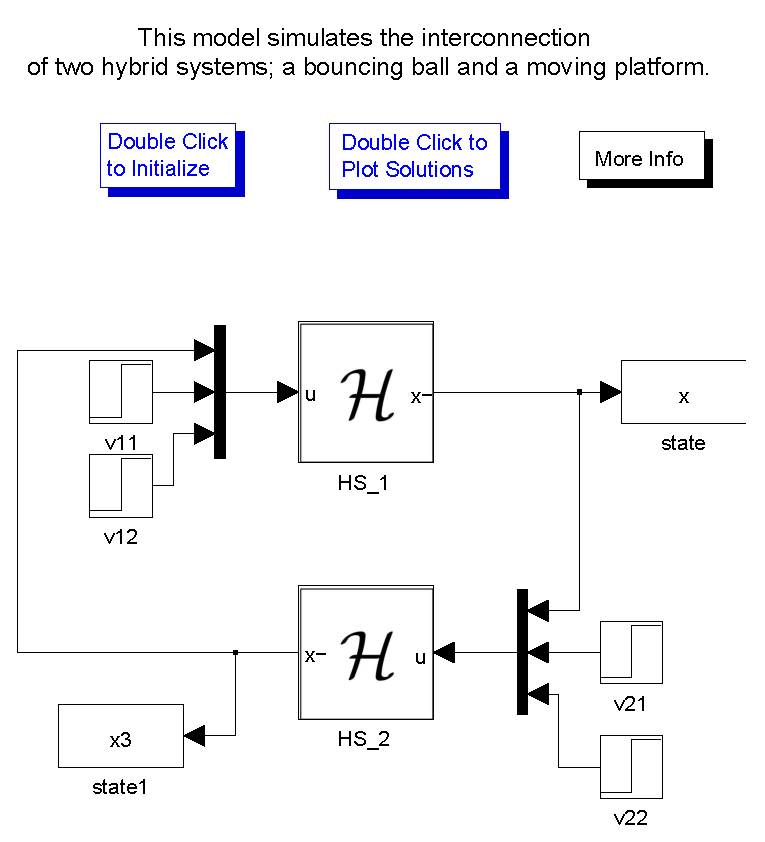
\includegraphics[width=.6\textwidth]{figures/Simulink/InterconnectionMdl.eps}}
   \caption{MATLAB/Simulink implementation of interconnected hybrid systems $\HS_1$ and
$\HS_2$}
\label{fig:interconnection-1}
  \end{center}
\end{figure}

\begin{figure}[ht!]
  \begin{center}
  \psfrag{flows [t]}[c]{flows [$t$]}
  \psfrag{jumps [j]}[c]{jumps [$j$]}
  \psfrag{xi1, eta1}[c]{$\xi_1, \eta_1$}
  \psfrag{xi2, eta2}[c]{$\xi_2, \eta_2$}
    {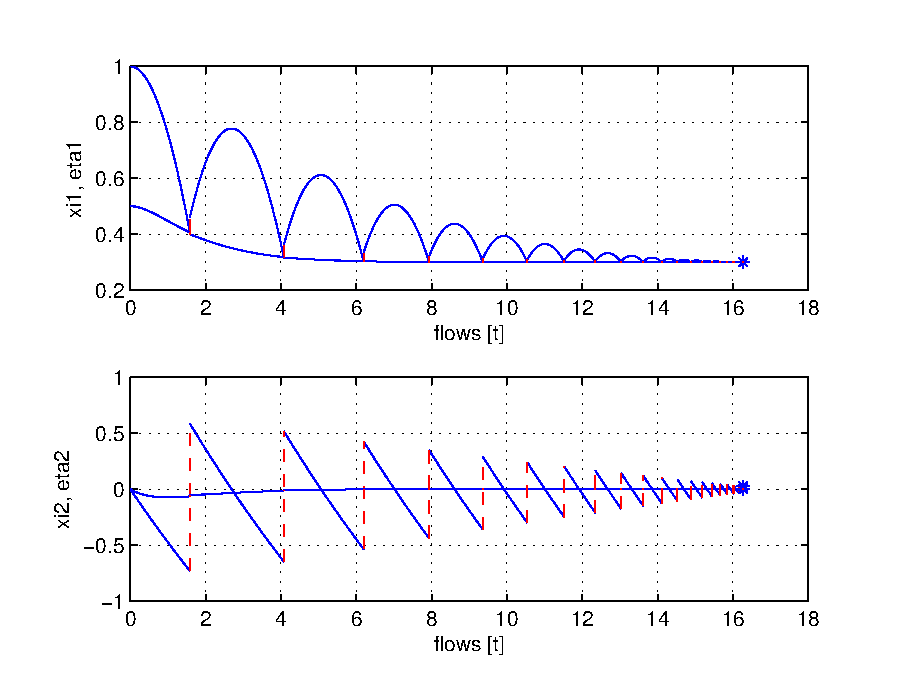
\includegraphics[width=.8\textwidth]{figures/Examples/InterconnectionH1H2.eps}}
   \caption{Solution of Example~\ref{ex:interconnection1}: height and velocity}
\label{fig:interconnection-2}
  \end{center}
\end{figure}

%\begin{figure}[ht]
%  \begin{center}
%  \psfrag{flows [t]}[c]{flows [$t$]}
%  \psfrag{jumps [j]}[c]{jumps [$j$]}
%  \psfrag{xi1}[c]{$\xi_1$}
%    {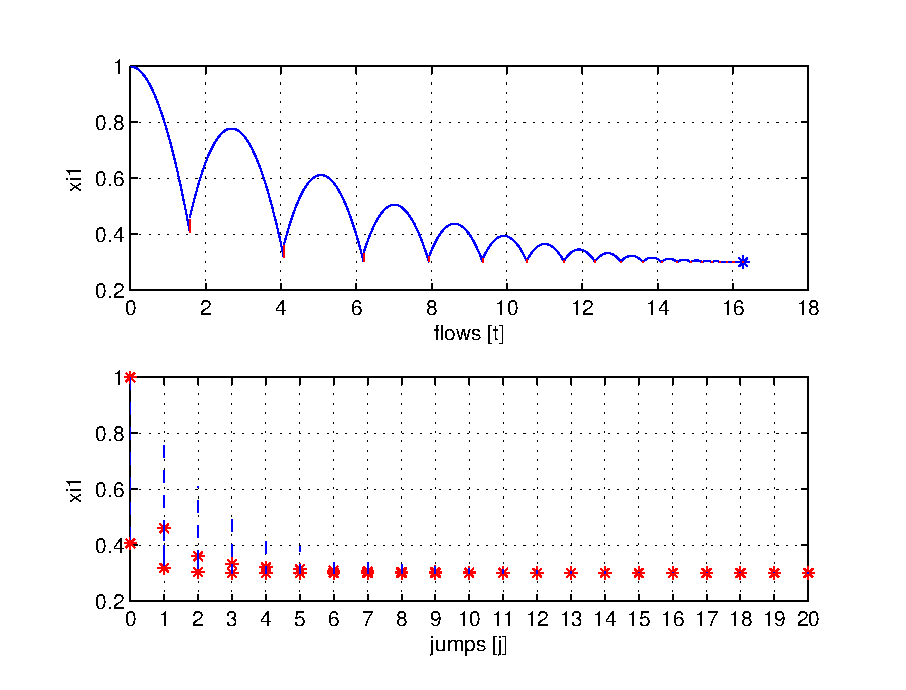
\includegraphics[width=.8\textwidth]{figures/Examples/InterconnectionH1.eps}}
%   \caption{Solution of Example~\ref{ex:interconnection1} for system $\HS_1$: height}
%\label{fig:interconnection-3}
%  \end{center}
%\end{figure}
%
%\begin{figure}[ht]
%  \begin{center}
%  \psfrag{flows [t]}[c]{flows [$t$]}
%  \psfrag{jumps [j]}[c]{jumps [$j$]}
%  \psfrag{xi2}[c]{$\xi_2$}
%    {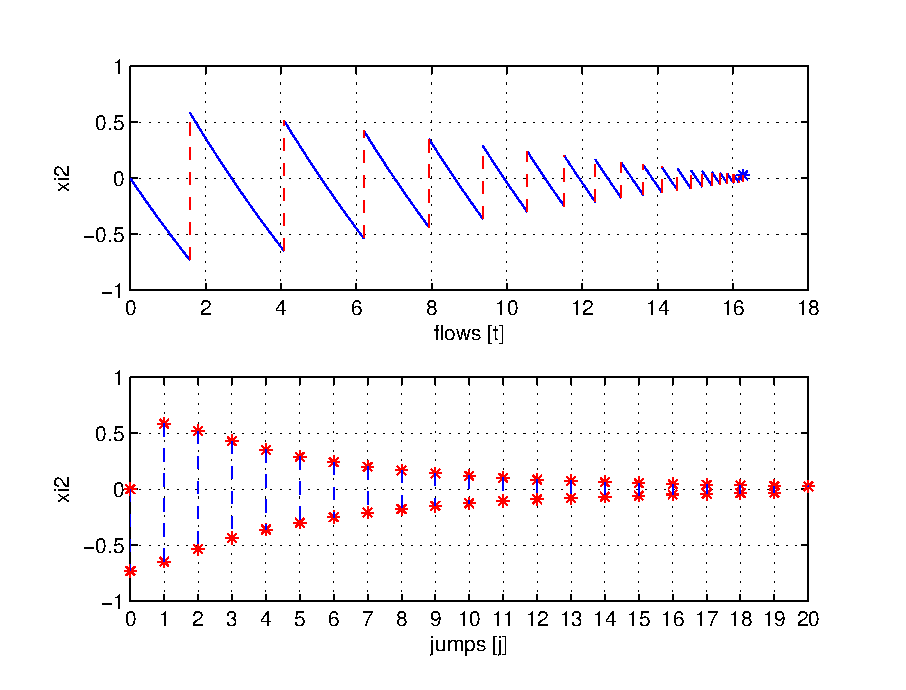
\includegraphics[width=.8\textwidth]{figures/Examples/InterconnectionH1velocity.eps}}
%   \caption{Solution of Example~\ref{ex:interconnection1} for system $\HS_1$: velocity}
%\label{fig:interconnection-4}
%  \end{center}
%\end{figure}

\begin{figure}[ht]
  \centering
  \psfrag{flows [t]}[c]{flows [$t$]}
  \psfrag{jumps [j]}[c]{jumps [$j$]}
  \psfrag{xi1}[c]{$\xi_1$}
  \psfrag{xi2}[c]{$\xi_2$}
\subfigure[Height]{
    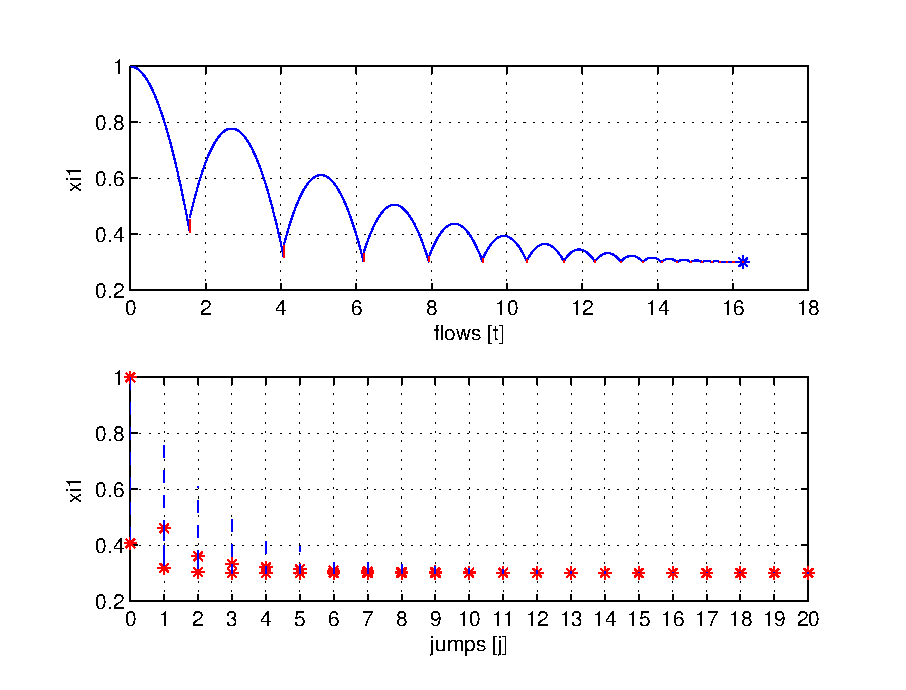
\includegraphics[width=.45\textwidth]{figures/Examples/InterconnectionH1.eps}
\label{fig:interconnection-3}}
\qquad
\subfigure[Velocity]{
    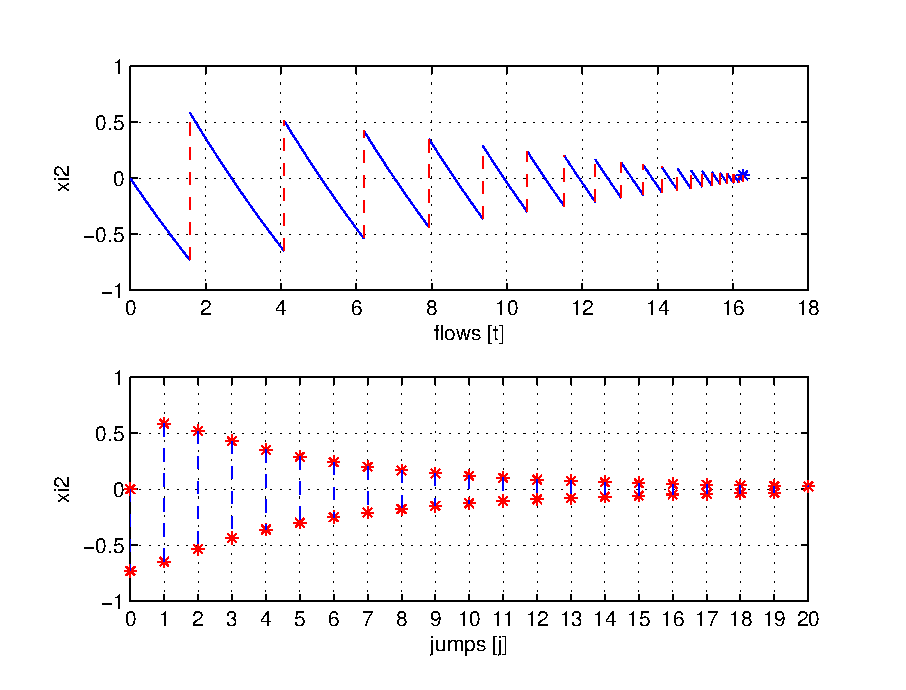
\includegraphics[width=.45\textwidth]{figures/Examples/InterconnectionH1velocity.eps}
\label{fig:interconnection-4}}
\caption{Solution of Example \ref{ex:interconnection1} for system $\HS_1$}
\end{figure}

%\begin{figure}[ht]
%  \begin{center}
%  \psfrag{flows [t]}[c]{flows [$t$]}
%  \psfrag{jumps [j]}[c]{jumps [$j$]}
%  \psfrag{eta1}[c]{$\eta_1$}
%    {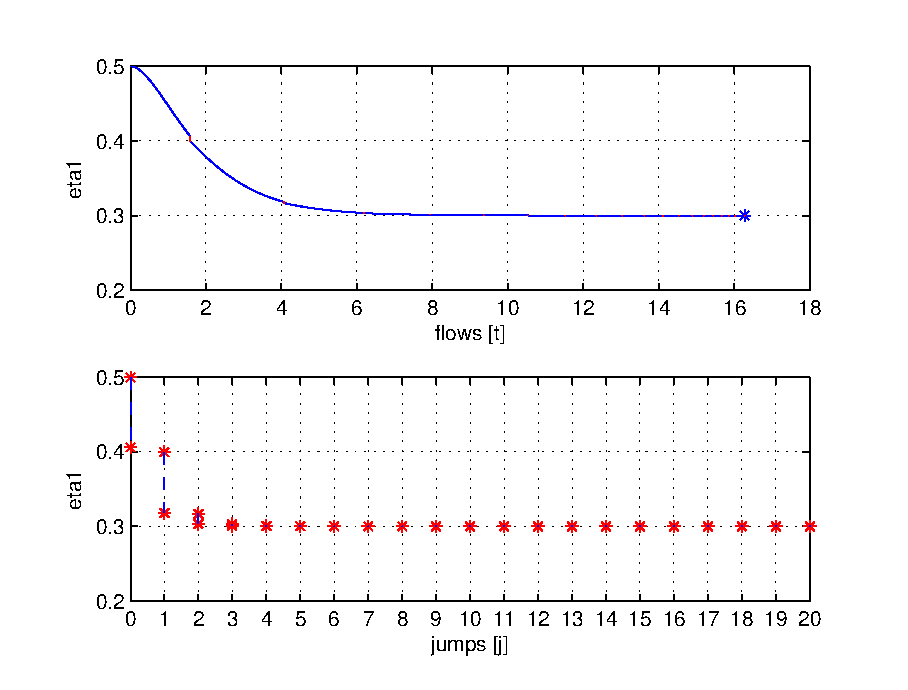
\includegraphics[width=.8\textwidth]{figures/Examples/InterconnectionH2.eps}}
%   \caption{Solution of Example~\ref{ex:interconnection1} for system $\HS_2$: height}
%\label{fig:interconnection-5}
%  \end{center}
%\end{figure}
%
%\begin{figure}[ht]
%  \begin{center}
%  \psfrag{flows [t]}[c]{flows [$t$]}
%  \psfrag{jumps [j]}[c]{jumps [$j$]}
%  \psfrag{eta2}[c]{$\eta_2$}
%    {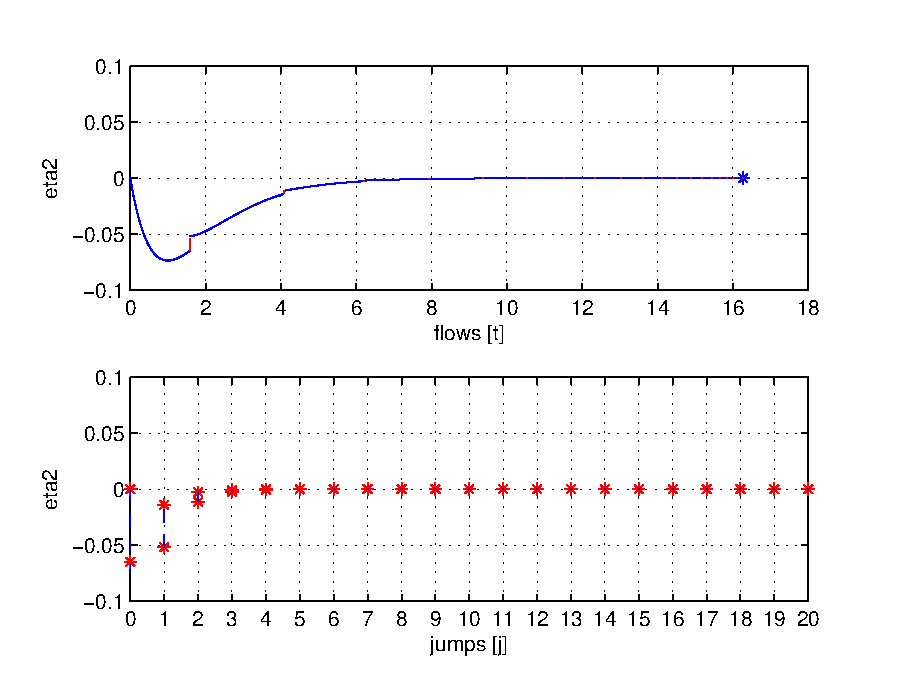
\includegraphics[width=.8\textwidth]{figures/Examples/InterconnectionH2velocity.eps}}
%   \caption{Solution of Example~\ref{ex:interconnection1} for system $\HS_2$: velocity}
%\label{fig:interconnection-6}
%  \end{center}
%\end{figure}

\begin{figure}[ht]
  \centering
  \psfrag{flows [t]}[c]{flows [$t$]}
  \psfrag{jumps [j]}[c]{jumps [$j$]}
  \psfrag{eta1}[c]{$\eta_1$}
  \psfrag{eta2}[c]{$\eta_2$}
\subfigure[Height]{
    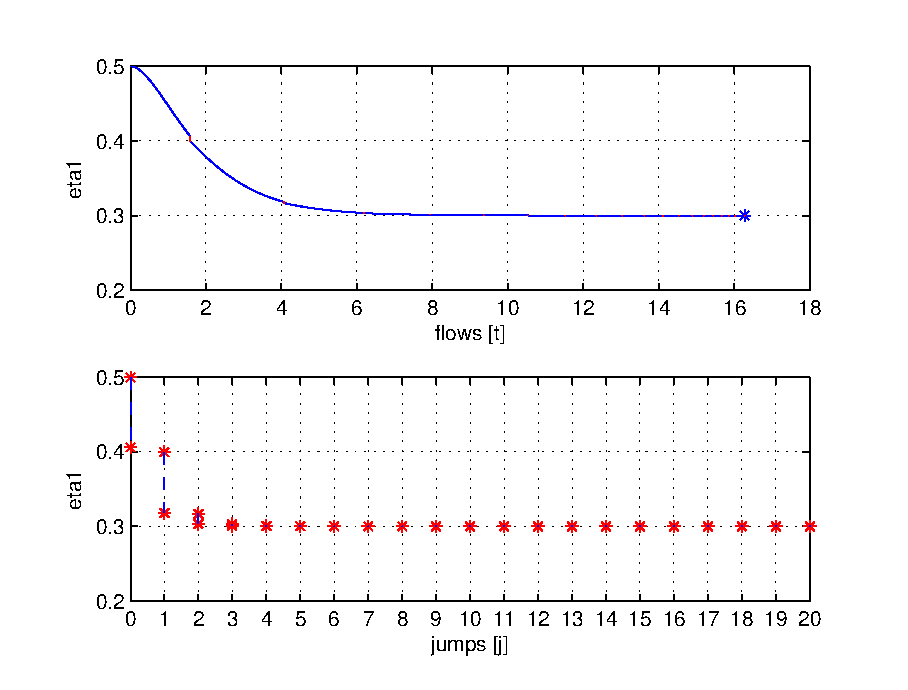
\includegraphics[width=.45\textwidth]{figures/Examples/InterconnectionH2.eps}
\label{fig:interconnection-5}}
\qquad
\subfigure[Velocity]{
    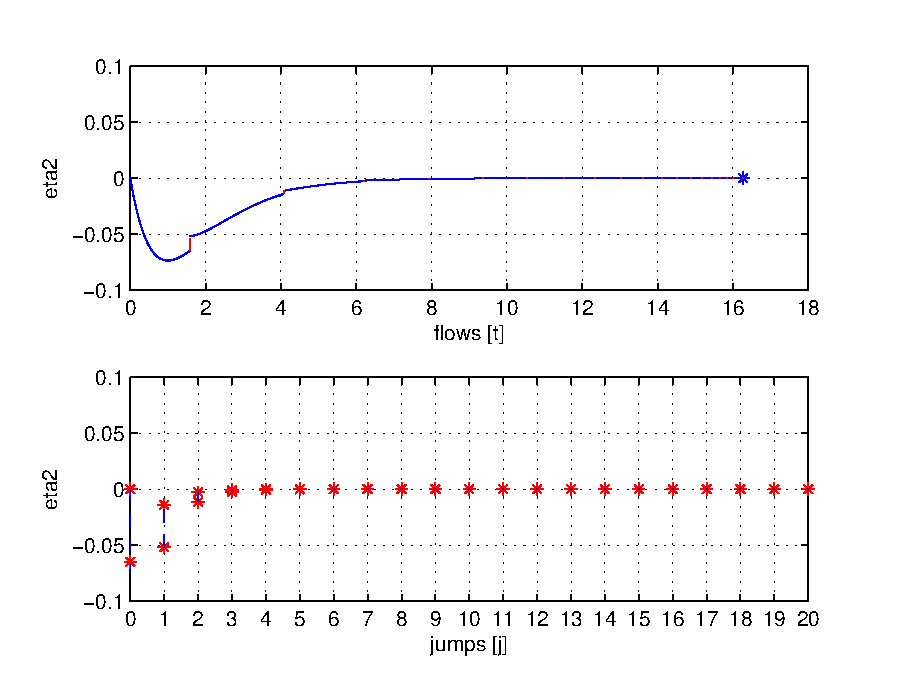
\includegraphics[width=.45\textwidth]{figures/Examples/InterconnectionH2velocity.eps}
\label{fig:interconnection-6}}
\caption{Solution of Example~\ref{ex:interconnection1} for system $\HS_2$}
\end{figure}

% Set the location for MATLAB files included via the "\code" command.
\codeLocation{Matlab2tex_1_6}

\begin{itemize}
\item For hybrid system $\HS_1$:

\code{f.m}
\code{C.m}
\code{g.m}
\code{D.m}

% Flow map
% %\scriptsize
% % This file was automatically created from the m-file 
% "m2tex.m" written by USL. 
% The fontencoding in this file is UTF-8. 
%  
% You will need to include the following two packages in 
% your LaTeX-Main-File. 
%  
% \usepackage{color} 
% \usepackage{fancyvrb} 
%  
% It is advised to use the following option for Inputenc 
% \usepackage[utf8]{inputenc} 
%  
  
% definition of matlab colors: 
\definecolor{mblue}{rgb}{0,0,1} 
\definecolor{mgreen}{rgb}{0.13333,0.5451,0.13333} 
\definecolor{mred}{rgb}{0.62745,0.12549,0.94118} 
\definecolor{mgrey}{rgb}{0.5,0.5,0.5} 
\definecolor{mdarkgrey}{rgb}{0.25,0.25,0.25} 
  
\DefineShortVerb[fontfamily=courier,fontseries=m]{\$} 
\DefineShortVerb[fontfamily=courier,fontseries=b]{\#} 
  
\noindent                    
 \hspace*{-1.6em}{\scriptsize 1}$  $\color{mblue}$function$\color{black}$ xdot = f(x, u, gamma)$\\
 \hspace*{-1.6em}{\scriptsize 2}$  $\\
 \hspace*{-1.6em}{\scriptsize 3}$  $\color{mgreen}#%%%%%%%%%%%%%%%%%%%%%%%%%%%%%%%%%%%%%%%%%%%%%%%%%%%%%%%%%%%%%%%%%%%%%%%%%%%#\color{black}$$\\
 \hspace*{-1.6em}{\scriptsize 4}$  $\color{mgreen}$% Matlab Function  Author: Ricardo Sanfelice $\color{black}$$\\
 \hspace*{-1.6em}{\scriptsize 5}$  $\color{mgreen}$% (Revised by Giampiero Campa)$\color{black}$$\\
 \hspace*{-1.6em}{\scriptsize 6}$  $\color{mgreen}$% (Revised by Pablo Nanez)$\color{black}$$\\
 \hspace*{-1.6em}{\scriptsize 7}$  $\color{mgreen}$%$\color{black}$$\\
 \hspace*{-1.6em}{\scriptsize 8}$  $\color{mgreen}$% Project: Simulation of a hybrid system (Bouncing Ball)$\color{black}$$\\
 \hspace*{-1.6em}{\scriptsize 9}$  $\color{mgreen}$%$\color{black}$$\\
 \hspace*{-2em}{\scriptsize 10}$  $\color{mgreen}$% Name: f.m$\color{black}$$\\
 \hspace*{-2em}{\scriptsize 11}$  $\color{mgreen}$%$\color{black}$$\\
 \hspace*{-2em}{\scriptsize 12}$  $\color{mgreen}$% Description: Flow map$\color{black}$$\\
 \hspace*{-2em}{\scriptsize 13}$  $\color{mgreen}$%$\color{black}$$\\
 \hspace*{-2em}{\scriptsize 14}$  $\color{mgreen}$% Version: 1.0$\color{black}$$\\
 \hspace*{-2em}{\scriptsize 15}$  $\color{mgreen}$% Required files: - $\color{black}$$\\
 \hspace*{-2em}{\scriptsize 16}$  $\color{mgreen}#%%%%%%%%%%%%%%%%%%%%%%%%%%%%%%%%%%%%%%%%%%%%%%%%%%%%%%%%%%%%%%%%%%%%%%%%%%%#\color{black}$$\\
 \hspace*{-2em}{\scriptsize 17}$  $\\
 \hspace*{-2em}{\scriptsize 18}$  $\\
 \hspace*{-2em}{\scriptsize 19}$  $\color{mgreen}$% flow map: xdot=f(x,u);$\color{black}$$\\
 \hspace*{-2em}{\scriptsize 20}$  xdot = [x(2); gamma];$\\ 
  
\UndefineShortVerb{\$} 
\UndefineShortVerb{\#}\label{scr:f}
% %\normalsize

% Flow set
% %\scriptsize
% % This file was automatically created from the m-file 
% "m2tex.m" written by USL. 
% The fontencoding in this file is UTF-8. 
%  
% You will need to include the following two packages in 
% your LaTeX-Main-File. 
%  
% \usepackage{color} 
% \usepackage{fancyvrb} 
%  
% It is advised to use the following option for Inputenc 
% \usepackage[utf8]{inputenc} 
%  
  
% definition of matlab colors: 
\definecolor{mblue}{rgb}{0,0,1} 
\definecolor{mgreen}{rgb}{0.13333,0.5451,0.13333} 
\definecolor{mred}{rgb}{0.62745,0.12549,0.94118} 
\definecolor{mgrey}{rgb}{0.5,0.5,0.5} 
\definecolor{mdarkgrey}{rgb}{0.25,0.25,0.25} 
  
\DefineShortVerb[fontfamily=courier,fontseries=m]{\$} 
\DefineShortVerb[fontfamily=courier,fontseries=b]{\#} 
  
\noindent                          
 \hspace*{-1.6em}{\scriptsize 1}$  $\color{mblue}$function$\color{black}$ v  = C(x, u)$\\
 \hspace*{-1.6em}{\scriptsize 2}$  $\color{mgreen}$%--------------------------------------------------------------------------$\color{black}$$\\
 \hspace*{-1.6em}{\scriptsize 3}$  $\color{mgreen}$% Matlab M-file Project: HyEQ Toolbox @  Hybrid Systems Laboratory (HSL),$\color{black}$$\\
 \hspace*{-1.6em}{\scriptsize 4}$  $\color{mgreen}$% https://hybrid.soe.ucsc.edu/software$\color{black}$$\\
 \hspace*{-1.6em}{\scriptsize 5}$  $\color{mgreen}$% http://hybridsimulator.wordpress.com/$\color{black}$$\\
 \hspace*{-1.6em}{\scriptsize 6}$  $\color{mgreen}$%--------------------------------------------------------------------------$\color{black}$$\\
 \hspace*{-1.6em}{\scriptsize 7}$  $\color{mgreen}$% Project: Simulation of a hybrid system$\color{black}$$\\
 \hspace*{-1.6em}{\scriptsize 8}$  $\color{mgreen}$% Description: Flow set$\color{black}$$\\
 \hspace*{-1.6em}{\scriptsize 9}$  $\color{mgreen}$%--------------------------------------------------------------------------$\color{black}$$\\
 \hspace*{-2em}{\scriptsize 10}$  $\color{mgreen}$%--------------------------------------------------------------------------$\color{black}$$\\
 \hspace*{-2em}{\scriptsize 11}$  $\color{mgreen}$%   See also HYEQSOLVER, PLOTARC, PLOTARC3, PLOTFLOWS, PLOTHARC,$\color{black}$$\\
 \hspace*{-2em}{\scriptsize 12}$  $\color{mgreen}$%   PLOTHARCCOLOR, PLOTHARCCOLOR3D, PLOTHYBRIDARC, PLOTJUMPS.$\color{black}$$\\
 \hspace*{-2em}{\scriptsize 13}$  $\color{mgreen}$%   Copyright @ Hybrid Systems Laboratory (HSL),$\color{black}$$\\
 \hspace*{-2em}{\scriptsize 14}$  $\color{mgreen}$%   Revision: 0.0.0.3 Date: 05/20/2015 3:42:00$\color{black}$$\\
 \hspace*{-2em}{\scriptsize 15}$  $\color{mgreen}$%$\color{black}$$\\
 \hspace*{-2em}{\scriptsize 16}$  $\color{mgreen}$% Check on flow conditions$\color{black}$$\\
 \hspace*{-2em}{\scriptsize 17}$  $\color{mgreen}$% E.g.,$\color{black}$$\\
 \hspace*{-2em}{\scriptsize 18}$  $\color{mgreen}$% if (x(1) >= u(1))  % flow condition$\color{black}$$\\
 \hspace*{-2em}{\scriptsize 19}$  $\color{mgreen}$%     v = 1;  % report flow$\color{black}$$\\
 \hspace*{-2em}{\scriptsize 20}$  $\color{mgreen}$% else$\color{black}$$\\
 \hspace*{-2em}{\scriptsize 21}$  $\color{mgreen}$%     v = 0;   % do not report flow$\color{black}$$\\
 \hspace*{-2em}{\scriptsize 22}$  $\color{mgreen}$% end$\color{black}$$\\
 \hspace*{-2em}{\scriptsize 23}$  $\\
 \hspace*{-2em}{\scriptsize 24}$  $\\
 \hspace*{-2em}{\scriptsize 25}$  v = 1; $\color{mgreen}$% report flow$\color{black}$$\\
 \hspace*{-2em}{\scriptsize 26}$  $\\ 
  
\UndefineShortVerb{\$} 
\UndefineShortVerb{\#}\label{scr:C}
% %\normalsize

% Jump map
% %\scriptsize
% % This file was automatically created from the m-file 
% "m2tex.m" written by USL. 
% The fontencoding in this file is UTF-8. 
%  
% You will need to include the following two packages in 
% your LaTeX-Main-File. 
%  
% \usepackage{color} 
% \usepackage{fancyvrb} 
%  
% It is advised to use the following option for Inputenc 
% \usepackage[utf8]{inputenc} 
%  
  
% definition of matlab colors: 
\definecolor{mblue}{rgb}{0,0,1} 
\definecolor{mgreen}{rgb}{0.13333,0.5451,0.13333} 
\definecolor{mred}{rgb}{0.62745,0.12549,0.94118} 
\definecolor{mgrey}{rgb}{0.5,0.5,0.5} 
\definecolor{mdarkgrey}{rgb}{0.25,0.25,0.25} 
  
\DefineShortVerb[fontfamily=courier,fontseries=m]{\$} 
\DefineShortVerb[fontfamily=courier,fontseries=b]{\#} 
  
\noindent   
 \hspace*{-1.6em}{\scriptsize 1}$  $\color{mblue}$function$\color{black}$ xplus = g(x, u, lambda)$\\
 \hspace*{-1.6em}{\scriptsize 2}$  $\color{mgreen}$% jump map$\color{black}$$\\
 \hspace*{-1.6em}{\scriptsize 3}$  xplus = [u(1); -lambda*x(2)];$\\ 
  
\UndefineShortVerb{\$} 
\UndefineShortVerb{\#}\label{scr:g}
% %\normalsize

% Jump set
% %\scriptsize
% % This file was automatically created from the m-file 
% "m2tex.m" written by USL. 
% The fontencoding in this file is UTF-8. 
%  
% You will need to include the following two packages in 
% your LaTeX-Main-File. 
%  
% \usepackage{color} 
% \usepackage{fancyvrb} 
%  
% It is advised to use the following option for Inputenc 
% \usepackage[utf8]{inputenc} 
%  
  
% definition of matlab colors: 
\definecolor{mblue}{rgb}{0,0,1} 
\definecolor{mgreen}{rgb}{0.13333,0.5451,0.13333} 
\definecolor{mred}{rgb}{0.62745,0.12549,0.94118} 
\definecolor{mgrey}{rgb}{0.5,0.5,0.5} 
\definecolor{mdarkgrey}{rgb}{0.25,0.25,0.25} 
  
\DefineShortVerb[fontfamily=courier,fontseries=m]{\$} 
\DefineShortVerb[fontfamily=courier,fontseries=b]{\#} 
  
\noindent                         
 \hspace*{-1.6em}{\scriptsize 1}$  $\color{mblue}$function$\color{black}$ v  = D(x, u) $\\
 \hspace*{-1.6em}{\scriptsize 2}$  $\\
 \hspace*{-1.6em}{\scriptsize 3}$  $\color{mgreen}#%%%%%%%%%%%%%%%%%%%%%%%%%%%%%%%%%%%%%%%%%%%%%%%%%%%%%%%%%%%%%%%%%%%%%%%%%%%#\color{black}$$\\
 \hspace*{-1.6em}{\scriptsize 4}$  $\color{mgreen}$% Matlab Function  Author: Ricardo Sanfelice $\color{black}$$\\
 \hspace*{-1.6em}{\scriptsize 5}$  $\color{mgreen}$% (Revised by Giampiero Campa)$\color{black}$$\\
 \hspace*{-1.6em}{\scriptsize 6}$  $\color{mgreen}$% (Revised by Pablo Nanez)$\color{black}$$\\
 \hspace*{-1.6em}{\scriptsize 7}$  $\color{mgreen}$%$\color{black}$$\\
 \hspace*{-1.6em}{\scriptsize 8}$  $\color{mgreen}$% Project: Simulation of a hybrid system (Bouncing ball)$\color{black}$$\\
 \hspace*{-1.6em}{\scriptsize 9}$  $\color{mgreen}$%$\color{black}$$\\
 \hspace*{-2em}{\scriptsize 10}$  $\color{mgreen}$% Name: D.m$\color{black}$$\\
 \hspace*{-2em}{\scriptsize 11}$  $\color{mgreen}$%$\color{black}$$\\
 \hspace*{-2em}{\scriptsize 12}$  $\color{mgreen}$% Description: Jump set$\color{black}$$\\
 \hspace*{-2em}{\scriptsize 13}$  $\color{mgreen}$%$\color{black}$$\\
 \hspace*{-2em}{\scriptsize 14}$  $\color{mgreen}$% Version: 1.0$\color{black}$$\\
 \hspace*{-2em}{\scriptsize 15}$  $\color{mgreen}$% Required files: - $\color{black}$$\\
 \hspace*{-2em}{\scriptsize 16}$  $\color{mgreen}#%%%%%%%%%%%%%%%%%%%%%%%%%%%%%%%%%%%%%%%%%%%%%%%%%%%%%%%%%%%%%%%%%%%%%%%%%%%#\color{black}$$\\
 \hspace*{-2em}{\scriptsize 17}$  $\\
 \hspace*{-2em}{\scriptsize 18}$  xtemp = zeros(2,1);$\\
 \hspace*{-2em}{\scriptsize 19}$  xtemp = x;$\\
 \hspace*{-2em}{\scriptsize 20}$  $\\
 \hspace*{-2em}{\scriptsize 21}$  $\color{mblue}$if$\color{black}$ (xtemp(1) <= u(1)) && (xtemp(2) <= 0)  $\color{mgreen}$% jump condition$\color{black}$$\\
 \hspace*{-2em}{\scriptsize 22}$      v = 1;  $\color{mgreen}$% report jump$\color{black}$$\\
 \hspace*{-2em}{\scriptsize 23}$  $\color{mblue}$else$\color{black}$$\\
 \hspace*{-2em}{\scriptsize 24}$      v = 0;   $\color{mgreen}$% do not report jump$\color{black}$$\\
 \hspace*{-2em}{\scriptsize 25}$  $\color{mblue}$end$\color{black}$$\\ 
  
\UndefineShortVerb{\$} 
\UndefineShortVerb{\#}\label{scr:D}
% %\normalsize

\item For hybrid system $\HS_2$:

\code{f2.m}
\code{C2.m}
\code{g2.m}
\code{D2.m}

% Flow map
% %\scriptsize
% % This file was automatically created from the m-file 
% "m2tex.m" written by USL. 
% The fontencoding in this file is UTF-8. 
%  
% You will need to include the following two packages in 
% your LaTeX-Main-File. 
%  
% \usepackage{color} 
% \usepackage{fancyvrb} 
%  
% It is advised to use the following option for Inputenc 
% \usepackage[utf8]{inputenc} 
%  
  
% definition of matlab colors: 
\definecolor{mblue}{rgb}{0,0,1} 
\definecolor{mgreen}{rgb}{0.13333,0.5451,0.13333} 
\definecolor{mred}{rgb}{0.62745,0.12549,0.94118} 
\definecolor{mgrey}{rgb}{0.5,0.5,0.5} 
\definecolor{mdarkgrey}{rgb}{0.25,0.25,0.25} 
  
\DefineShortVerb[fontfamily=courier,fontseries=m]{\$} 
\DefineShortVerb[fontfamily=courier,fontseries=b]{\#} 
  
\noindent            
 \hspace*{-1.6em}{\scriptsize 1}$  $\color{mblue}$function$\color{black}$ xdot = f(x, u)$\\
 \hspace*{-1.6em}{\scriptsize 2}$  $\color{mgreen}$% state$\color{black}$$\\
 \hspace*{-1.6em}{\scriptsize 3}$  eta1 = x(1);$\\
 \hspace*{-1.6em}{\scriptsize 4}$  eta2 = x(2);$\\
 \hspace*{-1.6em}{\scriptsize 5}$  $\color{mgreen}$%input$\color{black}$$\\
 \hspace*{-1.6em}{\scriptsize 6}$  y1 = u(1);$\\
 \hspace*{-1.6em}{\scriptsize 7}$  v21 = u(2);$\\
 \hspace*{-1.6em}{\scriptsize 8}$  v22 = u(3);$\\
 \hspace*{-1.6em}{\scriptsize 9}$  $\color{mgreen}$% flow map$\color{black}$$\\
 \hspace*{-2em}{\scriptsize 10}$  eta1dot = eta2;$\\
 \hspace*{-2em}{\scriptsize 11}$  eta2dot = -eta1-2*eta2+v21;$\\
 \hspace*{-2em}{\scriptsize 12}$  xdot = [eta1dot;eta2dot];$\\ 
  
\UndefineShortVerb{\$} 
\UndefineShortVerb{\#}\label{scr:f2}
% %\normalsize

% Flow set
% %\scriptsize
% % This file was automatically created from the m-file 
% "m2tex.m" written by USL. 
% The fontencoding in this file is UTF-8. 
%  
% You will need to include the following two packages in 
% your LaTeX-Main-File. 
%  
% \usepackage{color} 
% \usepackage{fancyvrb} 
%  
% It is advised to use the following option for Inputenc 
% \usepackage[utf8]{inputenc} 
%  
  
% definition of matlab colors: 
\definecolor{mblue}{rgb}{0,0,1} 
\definecolor{mgreen}{rgb}{0.13333,0.5451,0.13333} 
\definecolor{mred}{rgb}{0.62745,0.12549,0.94118} 
\definecolor{mgrey}{rgb}{0.5,0.5,0.5} 
\definecolor{mdarkgrey}{rgb}{0.25,0.25,0.25} 
  
\DefineShortVerb[fontfamily=courier,fontseries=m]{\$} 
\DefineShortVerb[fontfamily=courier,fontseries=b]{\#} 
  
\noindent                             
 \hspace*{-1.6em}{\scriptsize 1}$  $\color{mblue}$function$\color{black}$ v  = C(x, u) $\\
 \hspace*{-1.6em}{\scriptsize 2}$  $\\
 \hspace*{-1.6em}{\scriptsize 3}$  $\color{mgreen}#%%%%%%%%%%%%%%%%%%%%%%%%%%%%%%%%%%%%%%%%%%%%%%%%%%%%%%%%%%%%%%%%%%%%%%%%%%%#\color{black}$$\\
 \hspace*{-1.6em}{\scriptsize 4}$  $\color{mgreen}$% Matlab Function  Author: Ricardo Sanfelice $\color{black}$$\\
 \hspace*{-1.6em}{\scriptsize 5}$  $\color{mgreen}$%$\color{black}$$\\
 \hspace*{-1.6em}{\scriptsize 6}$  $\color{mgreen}$% Project: Simulation of a hybrid system (interconnection)$\color{black}$$\\
 \hspace*{-1.6em}{\scriptsize 7}$  $\color{mgreen}$%$\color{black}$$\\
 \hspace*{-1.6em}{\scriptsize 8}$  $\color{mgreen}$% Name: C.m$\color{black}$$\\
 \hspace*{-1.6em}{\scriptsize 9}$  $\color{mgreen}$%$\color{black}$$\\
 \hspace*{-2em}{\scriptsize 10}$  $\color{mgreen}$% Description: Flow set$\color{black}$$\\
 \hspace*{-2em}{\scriptsize 11}$  $\color{mgreen}$%$\color{black}$$\\
 \hspace*{-2em}{\scriptsize 12}$  $\color{mgreen}$% Version: 1.0$\color{black}$$\\
 \hspace*{-2em}{\scriptsize 13}$  $\color{mgreen}$% Required files: - $\color{black}$$\\
 \hspace*{-2em}{\scriptsize 14}$  $\color{mgreen}#%%%%%%%%%%%%%%%%%%%%%%%%%%%%%%%%%%%%%%%%%%%%%%%%%%%%%%%%%%%%%%%%%%%%%%%%%%%#\color{black}$$\\
 \hspace*{-2em}{\scriptsize 15}$  $\\
 \hspace*{-2em}{\scriptsize 16}$  $\color{mgreen}$% state$\color{black}$$\\
 \hspace*{-2em}{\scriptsize 17}$  eta1 = x(1);$\\
 \hspace*{-2em}{\scriptsize 18}$  eta2 = x(2);$\\
 \hspace*{-2em}{\scriptsize 19}$  $\\
 \hspace*{-2em}{\scriptsize 20}$  $\color{mgreen}$%input$\color{black}$$\\
 \hspace*{-2em}{\scriptsize 21}$  y1 = u(1);$\\
 \hspace*{-2em}{\scriptsize 22}$  v21 = u(2);$\\
 \hspace*{-2em}{\scriptsize 23}$  v22 = u(3);$\\
 \hspace*{-2em}{\scriptsize 24}$  $\\
 \hspace*{-2em}{\scriptsize 25}$  $\color{mblue}$if$\color{black}$ (eta1 <= y1)  $\color{mgreen}$% flow condition$\color{black}$$\\
 \hspace*{-2em}{\scriptsize 26}$      v = 1;  $\color{mgreen}$% report flow$\color{black}$$\\
 \hspace*{-2em}{\scriptsize 27}$  $\color{mblue}$else$\color{black}$$\\
 \hspace*{-2em}{\scriptsize 28}$      v = 0;   $\color{mgreen}$% do not report flow$\color{black}$$\\
 \hspace*{-2em}{\scriptsize 29}$  $\color{mblue}$end$\color{black}$$\\ 
  
\UndefineShortVerb{\$} 
\UndefineShortVerb{\#}\label{scr:C2}
% %\normalsize

% Jump map
% %\scriptsize
% % This file was automatically created from the m-file 
% "m2tex.m" written by USL. 
% The fontencoding in this file is UTF-8. 
%  
% You will need to include the following two packages in 
% your LaTeX-Main-File. 
%  
% \usepackage{color} 
% \usepackage{fancyvrb} 
%  
% It is advised to use the following option for Inputenc 
% \usepackage[utf8]{inputenc} 
%  
  
% definition of matlab colors: 
\definecolor{mblue}{rgb}{0,0,1} 
\definecolor{mgreen}{rgb}{0.13333,0.5451,0.13333} 
\definecolor{mred}{rgb}{0.62745,0.12549,0.94118} 
\definecolor{mgrey}{rgb}{0.5,0.5,0.5} 
\definecolor{mdarkgrey}{rgb}{0.25,0.25,0.25} 
  
\DefineShortVerb[fontfamily=courier,fontseries=m]{\$} 
\DefineShortVerb[fontfamily=courier,fontseries=b]{\#} 
  
\begin{Verbatim}[commandchars=\$\{\},numbers=left,numbersep=2pt] 

    $textcolor{mblue}{function} xplus = g(x, u) 
     
    $textcolor{mgreen}{%%%%%%%%%%%%%%%%%%%%%%%%%%%%%%%%%%%%%%%%%%%%%%%%%%%%%%%%%%%%%%%%%%%%%%%%%%%} 
    $textcolor{mgreen} 
    $textcolor{mgreen} 
    $textcolor{mgreen} 
    $textcolor{mgreen} 
    $textcolor{mgreen}{% Version: 1.0} 
    $textcolor{mgreen}{% Required files: - } 
    $textcolor{mgreen}{%%%%%%%%%%%%%%%%%%%%%%%%%%%%%%%%%%%%%%%%%%%%%%%%%%%%%%%%%%%%%%%%%%%%%%%%%%%} 
     
    $textcolor{mgreen}{% state} 
    eta1 = x(1); 
    eta2 = x(2); 
     
    $textcolor{mgreen}{%input} 
    y1 = u(1); 
    v21 = u(2); 
    v22 = u(3); 
     
    $textcolor{mgreen}{% jump map} 
    eta1plus = y1-0.1*abs(eta2); 
    eta2plus = -0.8*abs(eta2)+v22; 
     
    xplus = [eta1plus;eta2plus];  
\end{Verbatim}  
  
\UndefineShortVerb{\$} 
\UndefineShortVerb{\#} 
 \label{scr:g2}
% %\normalsize

% Jump set
% %\scriptsize
% % This file was automatically created from the m-file 
% "m2tex.m" written by USL. 
% The fontencoding in this file is UTF-8. 
%  
% You will need to include the following two packages in 
% your LaTeX-Main-File. 
%  
% \usepackage{color} 
% \usepackage{fancyvrb} 
%  
% It is advised to use the following option for Inputenc 
% \usepackage[utf8]{inputenc} 
%  
  
% definition of matlab colors: 
\definecolor{mblue}{rgb}{0,0,1} 
\definecolor{mgreen}{rgb}{0.13333,0.5451,0.13333} 
\definecolor{mred}{rgb}{0.62745,0.12549,0.94118} 
\definecolor{mgrey}{rgb}{0.5,0.5,0.5} 
\definecolor{mdarkgrey}{rgb}{0.25,0.25,0.25} 
  
\DefineShortVerb[fontfamily=courier,fontseries=m]{\$} 
\DefineShortVerb[fontfamily=courier,fontseries=b]{\#} 
  
\noindent              
 \hspace*{-1.6em}{\scriptsize 1}$  $\color{mblue}$function$\color{black}$ v = D(x, u)$\\
 \hspace*{-1.6em}{\scriptsize 2}$  $\color{mgreen}$% state$\color{black}$$\\
 \hspace*{-1.6em}{\scriptsize 3}$  eta1 = x(1);$\\
 \hspace*{-1.6em}{\scriptsize 4}$  eta2 = x(2);$\\
 \hspace*{-1.6em}{\scriptsize 5}$  $\color{mgreen}$%input$\color{black}$$\\
 \hspace*{-1.6em}{\scriptsize 6}$  y1 = u(1);$\\
 \hspace*{-1.6em}{\scriptsize 7}$  v21 = u(2);$\\
 \hspace*{-1.6em}{\scriptsize 8}$  v22 = u(3);$\\
 \hspace*{-1.6em}{\scriptsize 9}$  $\color{mgreen}$% jump set$\color{black}$$\\
 \hspace*{-2em}{\scriptsize 10}$  $\color{mblue}$if$\color{black}$ (eta1 >= y1) $\color{mgreen}$% jump condition$\color{black}$$\\
 \hspace*{-2em}{\scriptsize 11}$      v = 1;  $\color{mgreen}$% report jump$\color{black}$$\\
 \hspace*{-2em}{\scriptsize 12}$  $\color{mblue}$else$\color{black}$$\\
 \hspace*{-2em}{\scriptsize 13}$      v = 0;   $\color{mgreen}$% do not report jump$\color{black}$$\\
 \hspace*{-2em}{\scriptsize 14}$  $\color{mblue}$end$\color{black}$$\\ 
  
\UndefineShortVerb{\$} 
\UndefineShortVerb{\#}\label{scr:D2}
% %\normalsize

\end{itemize}

A solution to the interconnection of hybrid systems $\HS_1$ and
$\HS_2$ with $T=18, J=20$, $rule =1$, is depicted in Figure~\ref{fig:interconnection-2}.
Both the projection onto $t$ and $j$ are shown. A solution to the hybrid system $\HS_1$ is
depicted in Figure~\ref{fig:interconnection-3} (height) and Figure~\ref{fig:interconnection-4}
(velocity). A solution to the hybrid system $\HS_2$ is depicted in
Figure~\ref{fig:interconnection-5} (height) and Figure~\ref{fig:interconnection-6} (velocity).

These simulations reflect the expected behavior of the interconnected hybrid systems. %Note that in order to implement these systems without premature stopping of the simulation, $\xi_1$ in $g_1$ and $\eta_1$ in $g_2$ can be changed to $u_1$ and $u_2$, respectively so that $\xi_1^+=u_1$ and $\eta_1^+=u_2$.

For MATLAB/Simulink files of this example, see \IfSAE{Examples/Example\_\ref{ex:interconnection1}}{Examples/Example\_1.6}.

\end{example}



\end{document}
